\documentclass[a4paper,10pt]{report} % or \documentclass[a4paper,12pt]{book}

\setlength{\parindent}{0pt}

\usepackage[top=2cm, bottom=2cm, left=2cm, right=2cm]{geometry}
\usepackage{graphicx}
\usepackage{hyperref}
\usepackage{afterpage}
\usepackage{booktabs}
\usepackage{float}
\usepackage{multirow}



% Title page information
\title{Future Timelines: Extraction and Visualization of Future-related Content From News Articles}
\author{Juwal Regev}
\date{\today} % Use \date{Specific Date} for a fixed date

\begin{document}

\maketitle

\begin{abstract}
In today's rapidly evolving world, maintaining a comprehensive overview of the future landscape is essential for staying competitive and making informed decisions. However, given the large volume of daily news, manually obtaining a thorough overview of an entity's future prospects is quite challenging. To address this, we present a system designed to automatically extract and summarize future-related information of a queried entity from news articles. Our approach utilizes a novel and publicly accessible multi-source dataset comprising 6,800 annotated sentences to fine-tune a language model to identify future-related sentences. We then use topic modeling to extract the main topics from the data and rank them by relevance as well as present them on an interactive timeline. User evaluations have shown that the timelines and summaries our system produces are useful. The system is available as a web application at: \url{https://chronicle2050.regevson.com}.
\end{abstract}

\tableofcontents

% Chapters
\chapter{Introduction}
A vast amount of news articles is published on the web every single day. A significant amount of those articles contains information that is predictive or related to future events. Extracting and analyzing such information regarding a specific entity would offer a comprehensive overview of its future prospects. However doing this manually is not feasible as one would have to sift through the articles line by line, identifying nuanced references to the future. Furthermore, this would have to be done regularly so as to always have the most up-to-date information. Thus, it is clear that an automated system, capable of extracting, processing and visualizing this information is needed. This system would be beneficial in a variety of different fields. From analyzing predictions related to stock market movements, monitoring corporate developments as well as gaining insights into market trends and emerging technologies, the potential applications are limitless. To address this problem, a system was developed for extracting, summarizing, ranking and visualizing future-related content within news collections. It consistes of five main components: 1) Data Retrieval and Preprocessing, 2) Classification, 3) Topic Modeling, 4) Postprocessing, 5) Time-Tagging. A visualization of the workflow can be seen in Figure X.
The process is initiated by a user providing an entity, whose future should be explored. The system then downloads and preprocesses thousands of news articles related to the provided entity. In the next step, a neural network classifier is employed to classify sentences as either being future-related or not. Following classification, these sentences are organized into distinct topics, which are then presented to the user in a segmented manner. Additionally, the topics are labeled with representative keywords that provide insight into the content of each cluster. To provide an even better overview, we incorporate a temporal perspective into the presentation of the results. We do this by analyzing the sentences for temporal expressions, extracting and normalizing them to a date and then mapping the sentences, ranked by their relevance, onto a timeline. 

In the following chapters, we will explore the system's components in detail, including their implementation details and the rationale behind the design decisions made. Our goal is to provide a comprehensive overview of the system, including the inner workings and theoretical foundations of the models employed.

In Chapter 2 we begin by conducting a comprehensive literature review of existing work on future information extraction and timeline generation, including both traditional and state-of-the-art approaches. This review allows us to identify the capabilities, limitations, and opportunities for advancement of each approach.

Chapter 3 delves into the task of data collection and preprocessing. It describes the different sources and methodology used to create a novel dataset of future-related and non-future related sentences and the process used to clean and label the sentences in the dataset.

In Chapter 4, we provide a detailed explanation of the inner workings of the Transformer architecture, alongside a breakdown of both the BERT and RoBERTa models, before finally arriving at the DistilROBERTa model, which is the model used in our classifier. This section therefore guides the reader from the foundational Transformer architecture to the final classification model.

Chapter 5 focuses on topic modeling, a technique that enables clustering of sentences into distinct topics. We briefly analyze conventional modeling approaches, discuss advanced alternatives like BERTopic, and showcase how BERTopic was configured for our system.

The extraction and normalization of temporal expressions is the topic of Chapter 6 where we explore the SUTime time tagger's capabilities and limitations.

Chapter 7 offers a comprehensive analysis of the system's implementation. We delve into implementation details of the frontend as well as the backend and explain the rationale behind the frameworks that were selected.

Finally, Chapter 8 summarizes the evaluation of the system based on metrics and user studies. This assessment provides valuable insights into the system's effectiveness and areas for further enhancement.

\begin{figure}[H]
\centering
% First image
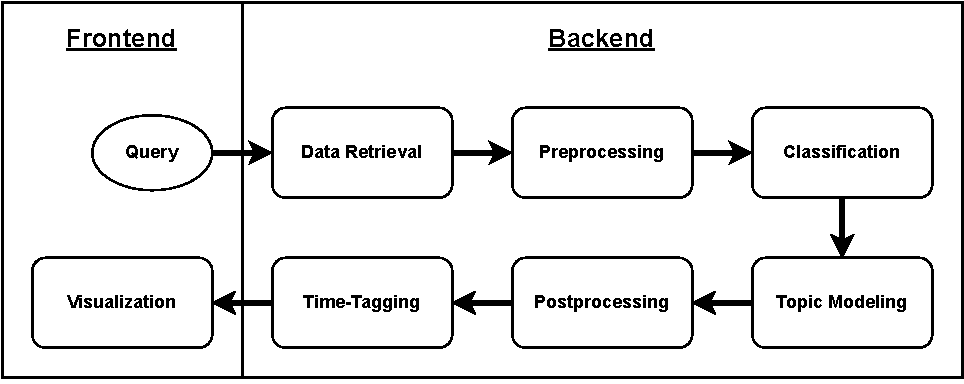
\includegraphics[width=13cm]{img/system.pdf}
\caption{Schematic Overview of the System's Data Processing Pipeline.}
\label{fig:archi}
\end{figure}



\chapter{Literature Review}

\section{Future Information Retrieval}
The field of information retrieval has made substantial progress in the last few decades, particularly in the context of future-oriented information retrieval and prediction. A notable beginning was marked by the visionary paper *Future Retrieval: A System for Predictive Information Search* (1990), which pioneered the concept of extracting temporal information from news sources and combining it with standard full-text retrieval to answer queries that integrate text and time. The paper's main contribution is defining the future retrieval problem and demonstrating its practicality through initial experiments and probabilistic models. \\

The methods for future Information Retrieval that followed, relied on time-taggers and predefined temporal expressions to extract data.
For example the year 2000 brought a temporal tagger (*Robust Temporal Processing of News*), that identified temporal expressions from text, tailored to news. It used hand-crafted rules as well as some machine learning to identify time expressions and assign normalized values.

The *ChronoSeeker system* also utilizes a rule-based approach to identify future-related sentences by employing chrono words (specific patterns and keywords typical of future-oriented sentences) combined with future years (e.g., "by the year 2040," "2010-2050") to formulate search queries. Sentences containing these chrono words are filtered from web pages and used to extract features for training a machine learning model that can accurately detect future-related sentences.
A similar approach was followed in *Analyzing Collective View of Future, Time-Referenced Events on the Web* , where future-related sentences are identified using regular expressions like: temp\_modifier+(the)year(s)+yyyy, which would match sentences like “In the year yyyy ...” or “... by the year yyyy.” 
*Ranking Related News Predictions* is another approach that uses hand crafted rules, this time with the TARSQI toolkit which extracts temporal expressions from documents. \\

Several studies have extended the traditional approach by analyzing obtained future-related sentences for distinctive characteristics and then doing classification based on those.

*Improving Retrieval of Future-Related Information in Text Collections* for example took an approach focusing on retrieving time-referenced and time-unreferenced predictions from text collections. Particularly the latter one is challenging as one has to move beyond rule-based methods for detection. The approach involves assembling document collections that represent past and future references. Then characteristic terms are identified that are prevalent in these collections. When analyzing a sentence, its classification as future-related or not is determined based on the presence of these characteristic terms.

*Computational Exploration of the Linguistic Structures of Future-Oriented Expression: Classification and Categorization* uses a combination of constituency grammar parsing, n-gram features, and 39 predefined syntactic rules to form features used to train an ADAGRAD classifier for detecting future-oriented sentences. *Automatic Extraction of References to Future Events from News Articles Using Semantic and Morphological Information* uses morphosemantic patterns as features, while *Extracting Predictive Statements with Their Scope from News Articles* classified clauses using features like POS tags and word co-occurrences to determine if a sentence refers to the future. Semantic role labeling was also employed for this purpose in *A Method for Extraction of Future Reference Sentences Based on Semantic Role  Labeling* \\

Some systems employed a predictive approach that analyzed past data to forecast future events.

*Predicting the News of Tomorrow Using Patterns in Web Search Queries* introduced PROFET, a method leveraging large-scale web resources like Google Trends to predict 100 terms that would dominate news headlines up to a week ahead. It underscored the potential of utilizing user search behavior as a predictive tool for future events.
The paper *Mining the Web to Predict Future Events* also analyzes historical news data to forecast significant occurrences in the future. News stories spanning over two decades were analyzed to extract event sequences. These sequences were then clustered together based on their shared topics using topic tracking algorithms. This resulted in the construction of event storylines. The storylines were then enriched with factual data from the web.

\section{Timeline Summarization}
In the timeline summarization line of research, which is also related to our study, content is grouped and ranked to form a timeline. For this there have also been multiple different approaches over the years. \\

*Automatic Generation of Overview Timelines (2000)* introduces a model for automatically creating timelines from text corpora. The process starts with extracting named entities and noun phrases from the timestamped articles. A chi-square test assesses the significance of term occurrences. Peaks are identified by finding runs of days with high chi-square scores. Terms with overlapping peak date ranges are clustered, representing related topics or events. Each cluster is labeled using the most prominent named entity and noun phrase. The clustering evaluation reveals disagreements on what constitutes a "topic".

The method proposed in *"Extracting Collective Expectations about the Future from Large Text Collections"* employs a time-tagger to identify and normalize temporal expressions in news articles. A probability distribution is assigned to each temporal expression to represent the uncertainty associated with the future event implied by the detected temporal expression. Subsequently, each sentence along with its corresponding temporal expression is represented as a bag of words and the assigned probability distribution. These representations are then clustered using a Gaussian Mixture Model to group similar future events based on their textual content and similar probability distributions.

*Temporal Summaries of News Topics* presented an approach to generate summaries that capture key events within a news topic over time, using probabilistic models for "novelty" and "usefulness". It showed that simple probabilistic models performed reasonably well, but not dramatically better than baseline models. *Query Based Event Extraction along a Timeline* further refined this concept by extracting sentences relevant to a query and placing them along a timeline based on their publication date. At each date the top N sentences are selected using special probabilistic measures like "interest" and "burstiness".

In the paper *Timeline Generation through Evolutionary Trans-Temporal Summarization,*  a new technique for Evolutionary Trans-Temporal Summarization is presented. It addresses the challenge of tracking the progression of news stories over time. Key steps include gathering time-stamped web documents, analyzing sentence dependencies within and across dates by using models for affinity and diversity among sentences to calculate their global and local ranking scores using DivRank (a variation of the PageRank algorithm). These scores help in constructing a ranking for sentences that are most important across the entire timeline and within individual dates. Based on the ranking, the most relevant sentences are selected to represent key points in the news evolution. \\

The first abstractive approach to timeline summarization came with *Abstractive Timeline Summarization*. Instead of identifying important sentences from a corpus and copying them directly into a timeline, this approach generates new sentences that combine information from various sources. It does this by first clustering sentences into topics using Affinity Propagation. The most frequently occurring date in each cluster is identified as the cluster's representative date. For each cluster, candidate summary sentences are generated using Multi-Sentence Compression, which fuses information from multiple sentences into a single sentence. The candidate sentences are then ranked based on date relevance, informativeness and linguistic quality. The top-ranked sentences are selected greedily to form the timeline summary. \\

More recently Multi-Timeline Summarization developments improve upon standard timeline summarization methods by generating multiple, high-quality and diverse timelines that summarize different stories. *Multi-TimeLine Summarization (MTLS): Improving Timeline Summarization by Generating Multiple Summaries* proposed an unsupervised method that clusters SBERT embeddings through Affinity Propagation to detect events. This is followed by the selection of important events. Events that frequently co-occur and reference each other are identified in an event linking step and will form their own timeline. For each timeline, only the exemplar sentence is taken from each constituent event and the top 3 frequent non-stop words in each timeline are extracted to characterize the timeline topic.



\chapter{Dataset}
A classifier should be developed that is capable of accurately classifying sentences as either future-related or non-future-related. The classifier should be implemented in the form of a neural network. For these types of models to perform well, they have to be trained on a lot of data. Another thing to consider is that a neural network is only as good as its training data because it can only learn from the data it is given. 

That is why it's crucial that this data is diverse. When a network is trained on diverse data, it is exposed to different patterns within the data, which makes it understand the underlying structure and relationships within the data better. To make this concrete for us, it means that we should provide the network with sentences about different topics, with different words and different structures. That is why our approach to data gathering differs from traditional methods. Earlier strategies have frequently relied on extracting data using temporal expressions. However, this approach has its limitations. Predictions can often be intricate, lacking explicit dates or simple temporal cues. To address this, our dataset (which is publicly available\footnote{\url{https://github.com/regevson/chronicle2050}}) incorporates a rich variety of 6,800 manually labeled sentences. They have been collected from different sources without relying on specific queries, and therefore they exhibit unique lexical and structural features and contain a diverse set of topics. This enables our classifier to identify future-related content that does not contain standard temporal expressions hinting at future references.



\section{Sources of Dataset}
The be more concrete, our data originates from 4 different sources. A detailed breakdown of them is provided in Tab. \ref{tab:dataset}. In the following, the four sources are described in more detail.

\begin{table}[h]
  \centering
  \begin{tabular}{lccc}
    \toprule
    \multirow{2}{*}{\textbf{Sources}} & \multirow{2}{*}{\textbf{Positives}} & \multirow{2}{*}{\textbf{Negatives}} & \textbf{Sentences without} \\
    & & & \textbf{temporal expressions (\%)} \\
    \midrule
    Longbets & 448 & 0 & 20 \\
    Horizons & 51 & 62 & 84 \\
    ChatGPT & 305 & 305 & 70 \\
    News & 2501 & 3128 & 39 \\
    \bottomrule
    \textbf{Total} & \textbf{3305} & \textbf{3495} & \textbf{41} \\
  \bottomrule
  \end{tabular}
  \caption{Data Source Analysis: Count of Future-Related (Positive) vs. Non-Future-Related (Negative) Sentences, along with Percentage Free from Temporal Expressions.}
  \label{tab:dataset}
\end{table}

\subsection{LONGBETS}
First we looked for websites where users can make predictions about the future in the hopes of getting sentences from various different topics that give information about future events.
\begin{figure}
  \centering
  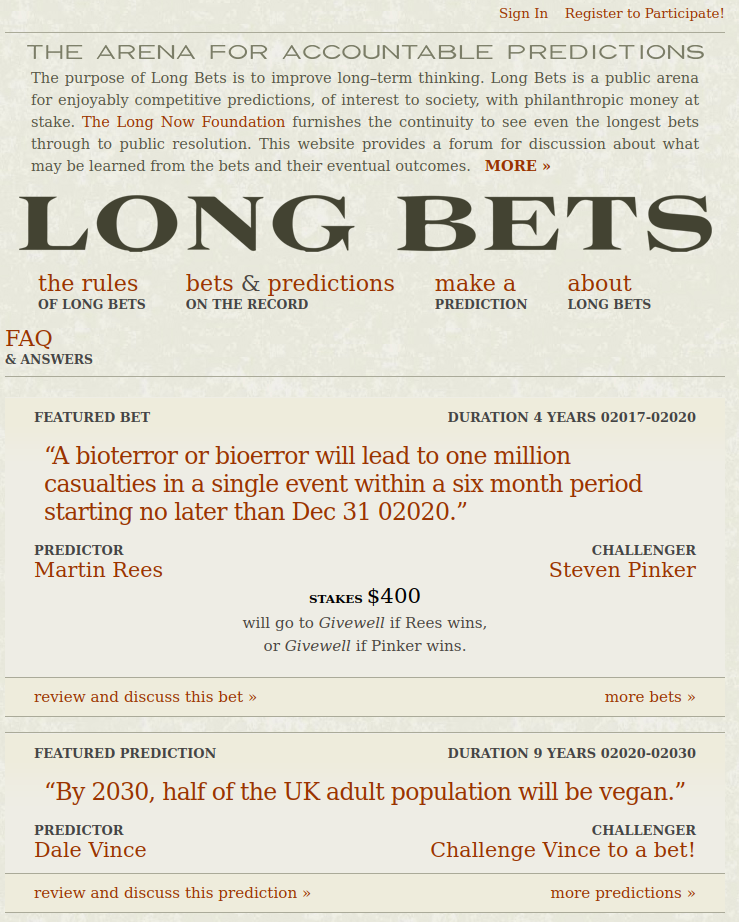
\includegraphics[height=10cm]{img/longbets.png}
  \caption{Screenshot of the LONGBETS website.}
  \label{fig:longbets}
\end{figure}
Longbets\footnote{\url{https://longbets.org}} is a platform where users are able to make predictions on various topics of interest.
The predictions on Longbets, spanning from realistic forecasts about politics and technology to the most audacious ones, extend all the way from the near future into the next century.
The prediction has to be summarized in one sentence. Additionally there is an option to give more context in the description section and even a possiblity to bet real money on the prediction.      
Here are several examples of sentences that have been scraped using the methodology described above:
\begin{itemize}
  \item \textit{"By 2030, commercial passengers will routinely fly in pilotless planes."}
  \item \textit{"Over the next ten years, we will make measurable global progress in all five areas of the human condition: food, access to clean water, health, education, and the price of energy."}
  \item \textit{"By 2029 no computer - or 'machine intelligence' - will have passed the Turing Test."}
\end{itemize}
    
\subsubsection{Analysis of the dataset}
Around one thousand predictions were obtained from Longbets. The majority of them is one sentence long.
\begin{itemize}
  \item 87\% of them contain a date
  \item 98\% of them contain \textit{"will"}
\end{itemize}

As we can see, this dataset does not meet the optimal criteria we established eralier, lacking the desirable attributes of diverse sentence structure and words. The majority of sentences have a structure like \textit{[... will ... -some date-]}. The content of the sentences does however represent different areas and topics.     
To create a balanced dataset, one thousand negative sentences scraped from news articles were added, which were subsequently reviewed manually. In order to maintain consistency with the positive sentences (which mostly contained dates), only negative sentences containing dates were selected.



\subsection{Horizons}
\begin{figure}
  \centering
  
\includegraphics[width=16cm]{img/horizons.png}
  \caption{Screenshot of the Horizons website.}
  \label{fig:horizons}
\end{figure}
Horizons\footnote{\url{https://radar.envisioning.io/horizons}} is more focused on emerging technologies. It is an "interactive visualization tool for discovering and learning about the technologies affecting our future". It introduces 100 emerging technologies by first describing them in detail and then focusing on their "Future Perspectives". For every technology the content of this subsection was scraped and stored. It was subsequently manually reviewed for future-related content.     
To make the dataset balanced, non-future-related sentences were added to the dataset. These sentences were taken from the technology description section of the same website.

\subsubsection{Analysis of the dataset}
Approximately 50 sentences were obtained as a result of this process. This is not a lot, however the quality of those sentences is high. Unlike the sentences scraped from longbets, these sentences have a more diverse structure with predictions being formed using words such as \textit{could}, \textit{may}, \textit{should}. The only drawback is that the sentences pertain solely to technology.

\begin{itemize}
  \item 23\% of them contain a date
  \item 47\% of them contain \textit{"will"}
\end{itemize}


\subsection{ChatGPT} % https://openai.com/blog/chatgpt, https://arxiv.org/pdf/2303.13367.pdf
ChatGPT is a groundbreaking language model developed by OpenAI in 2022. As a large-scale language model, it has been engineered to provide human-like responses to prompts and questions, mimicking a natural chat-based conversation. 

The architecture of ChatGPT is based on the GPT-3.5 model, but newer iterations like GPT-4 have since been introduced. Its underlying framework, the transformer architecture, plays a crucial role in enabling ChatGPT to understand and generate coherent and contextually appropriate responses.

By training on vast amounts of text data, ChatGPT has gained an impressive understanding of various domains, allowing it to engage in discussions on diverse topics. From addressing general knowledge questions to offering opinions and insights, ChatGPT demonstrates a remarkable ability to communicate effectively.

\subsubsection{ChatGPT for Training Data Generation}
ChatGPTs ability to generate responses in a chat-like format makes it an excellent tool for creating high-quality training data. By providing specific prompts to ChatGPT, developers can obtain targeted responses that align with their desired data requirements. This level of control allows for the generation of highly specific and tailored training data, which developers can use to fine-tune their models, enhancing the performance and applicability of their machine learning systems.

\subsubsection{Generating Future-related Sentences with ChatGPT}
As previously mentioned, the sentences extracted from sources such as \textit{Longbets} exhibit a notable similarity in structure, typically characterized by the presence of the word "will" followed by a future date. Recognizing the necessity for a more diverse range of sentence structures and vocabulary, the integration of ChatGPT became necessary. By leveraging the chatbots capabilities, a multitude of sentences encompassing varied sentence structures and lexical choices were generated. So the incorporation of ChatGPT effectively fulfilled the requirement for diversity in the training data, thereby improving the classifier's ability to handle a wider array of inputs. \\

In the following a subset of prompts are shown, that were used to generate the specific sentences:
\begin{itemize}
  \item \textit{"Give me 50 sentences about various topics, that contain future related information. Try to mix their sentence structure up and use different words."}
  \item \textit{"They should use words like 'could, 'would', 'may', 'might', …."}
  \item \textit{"They should be about two lines long."}
\end{itemize}

\subsection{News}
As already layed out, the classifier will ultimately need to classify sentences extracted from news articles. Therefore it makes sense for the dataset to be primarily composed of sentences originating from a news corpus. Manually searching for and extracting future-related sentences from news articles can be very time-consuming however. Consequently a bootstrapping approach was followed, which involved training the classifier initially only on the longbets, horizons, and chatgpt datasets. This first version of the classifier was then used to classify sentences extracted from 20,000 New York Times\footnote{\url{https://www.nytimes.com/}} articles.
Despite the limited amount of data used in the training process, the resulting classifier demonstrated an ability to make accurate predictions, making it much more viable to extract and review further predictions than extracting them manually. Moreover this gave the chance to identify the types of sentences that the model was uncertain about, which were then manually classified and incorporated into the training process.

\section{Annotation of Future-related Sentences}
\begin{figure}
  \centering
  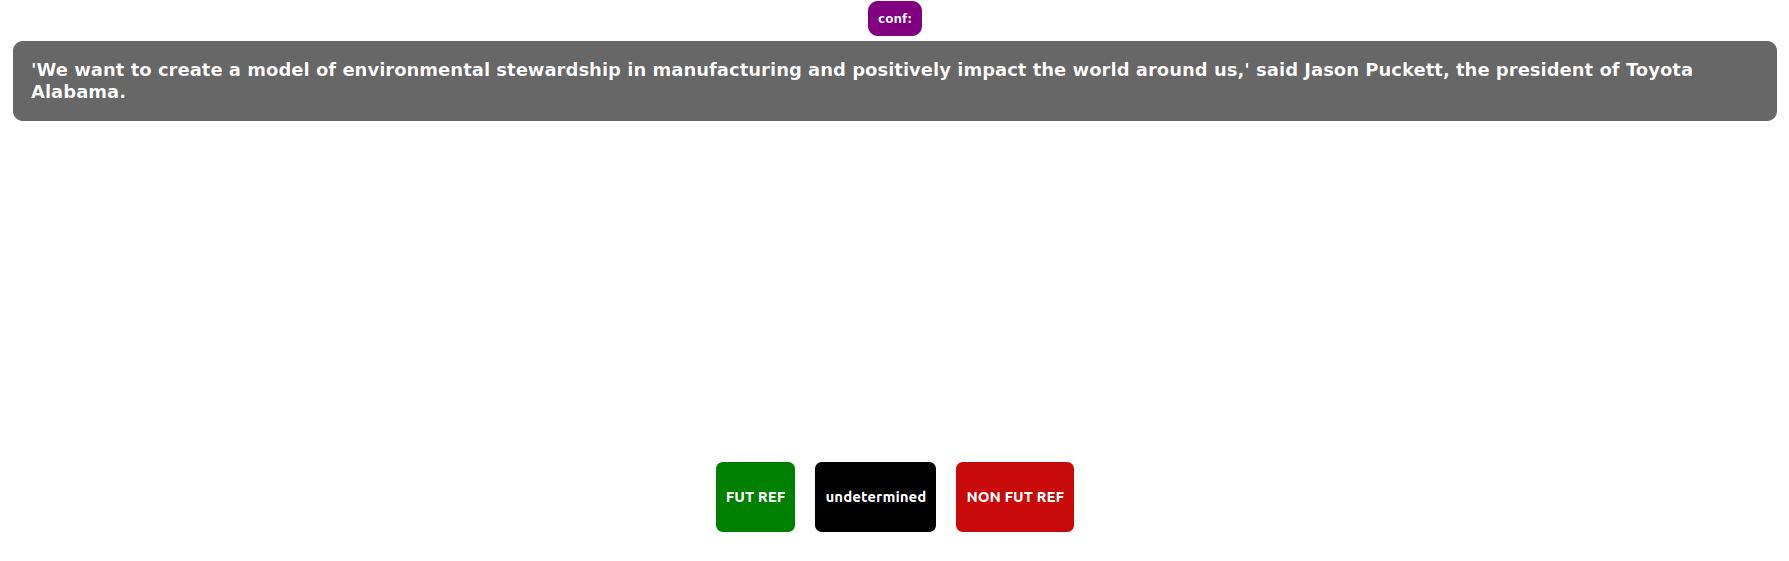
\includegraphics[width=16cm]{img/classification_website.png}
  \caption{Screenshot of the classification website.}
  \label{fig:classification_website}
\end{figure}
During the annotation process, manual annotation was required only for the news articles and horizons sources. All other sources, including longbets and chatgpt, consisted entirely of content related to the future. For the manual annotation task, approximately 3.5k sentences were labeled both as positive and negative.

To streamline the annotation process and enhance convenience, a simple website was developed specifically for this classification purpose. The website interface is designed to enable efficient labeling. At the top of the page, each sentence to be classified is displayed. Additionally, the confidence level of the classifier regarding the sentence's future-related content is presented below the sentence. This feature aims to provide insights into the classifier's performance regarding different sentence types.

Below the confidence level, three buttons are provided. The left button allows the user to label the sentence as containing future-related information. The middle button served as an option when the user is unsure about the appropriate category for the sentence. The right button enables the user to label the sentence as not containing future-related information.

This website-based approach significantly simplified the annotation process, offering a user-friendly environment for efficient classification. The straightforward layout of the website, coupled with its online availability, enables several people to work simultaneously on the classification task.

\chapter{Finetuned RoBERTa Classifier}
In this chapter, we delve into the core component of this project - the finetuned RoBERTa classifier. However, before delving into RoBERTa itself, it is essential to first understand the foundations upon which it is built. Therefore, we begin by examining the Transformer model and the BERT model, as RoBERTa builds upon their advancements. We explore the motivations behind selecting RoBERTa as the focus of our study and then proceed to unravel the intricacies of its architecture. This includes an in-depth exploration of its inner workings, the specifics of its training data, and the methodology employed during its training. Additionally, we investigate the process of tailoring the RoBERTa model to suit our unique classification task. Finally, we conclude our discussion by analyzing the evaluation and performance of the finetuned RoBERTa classifier.

\section{Transformer Architecture}
\begin{figure}
  \centering
  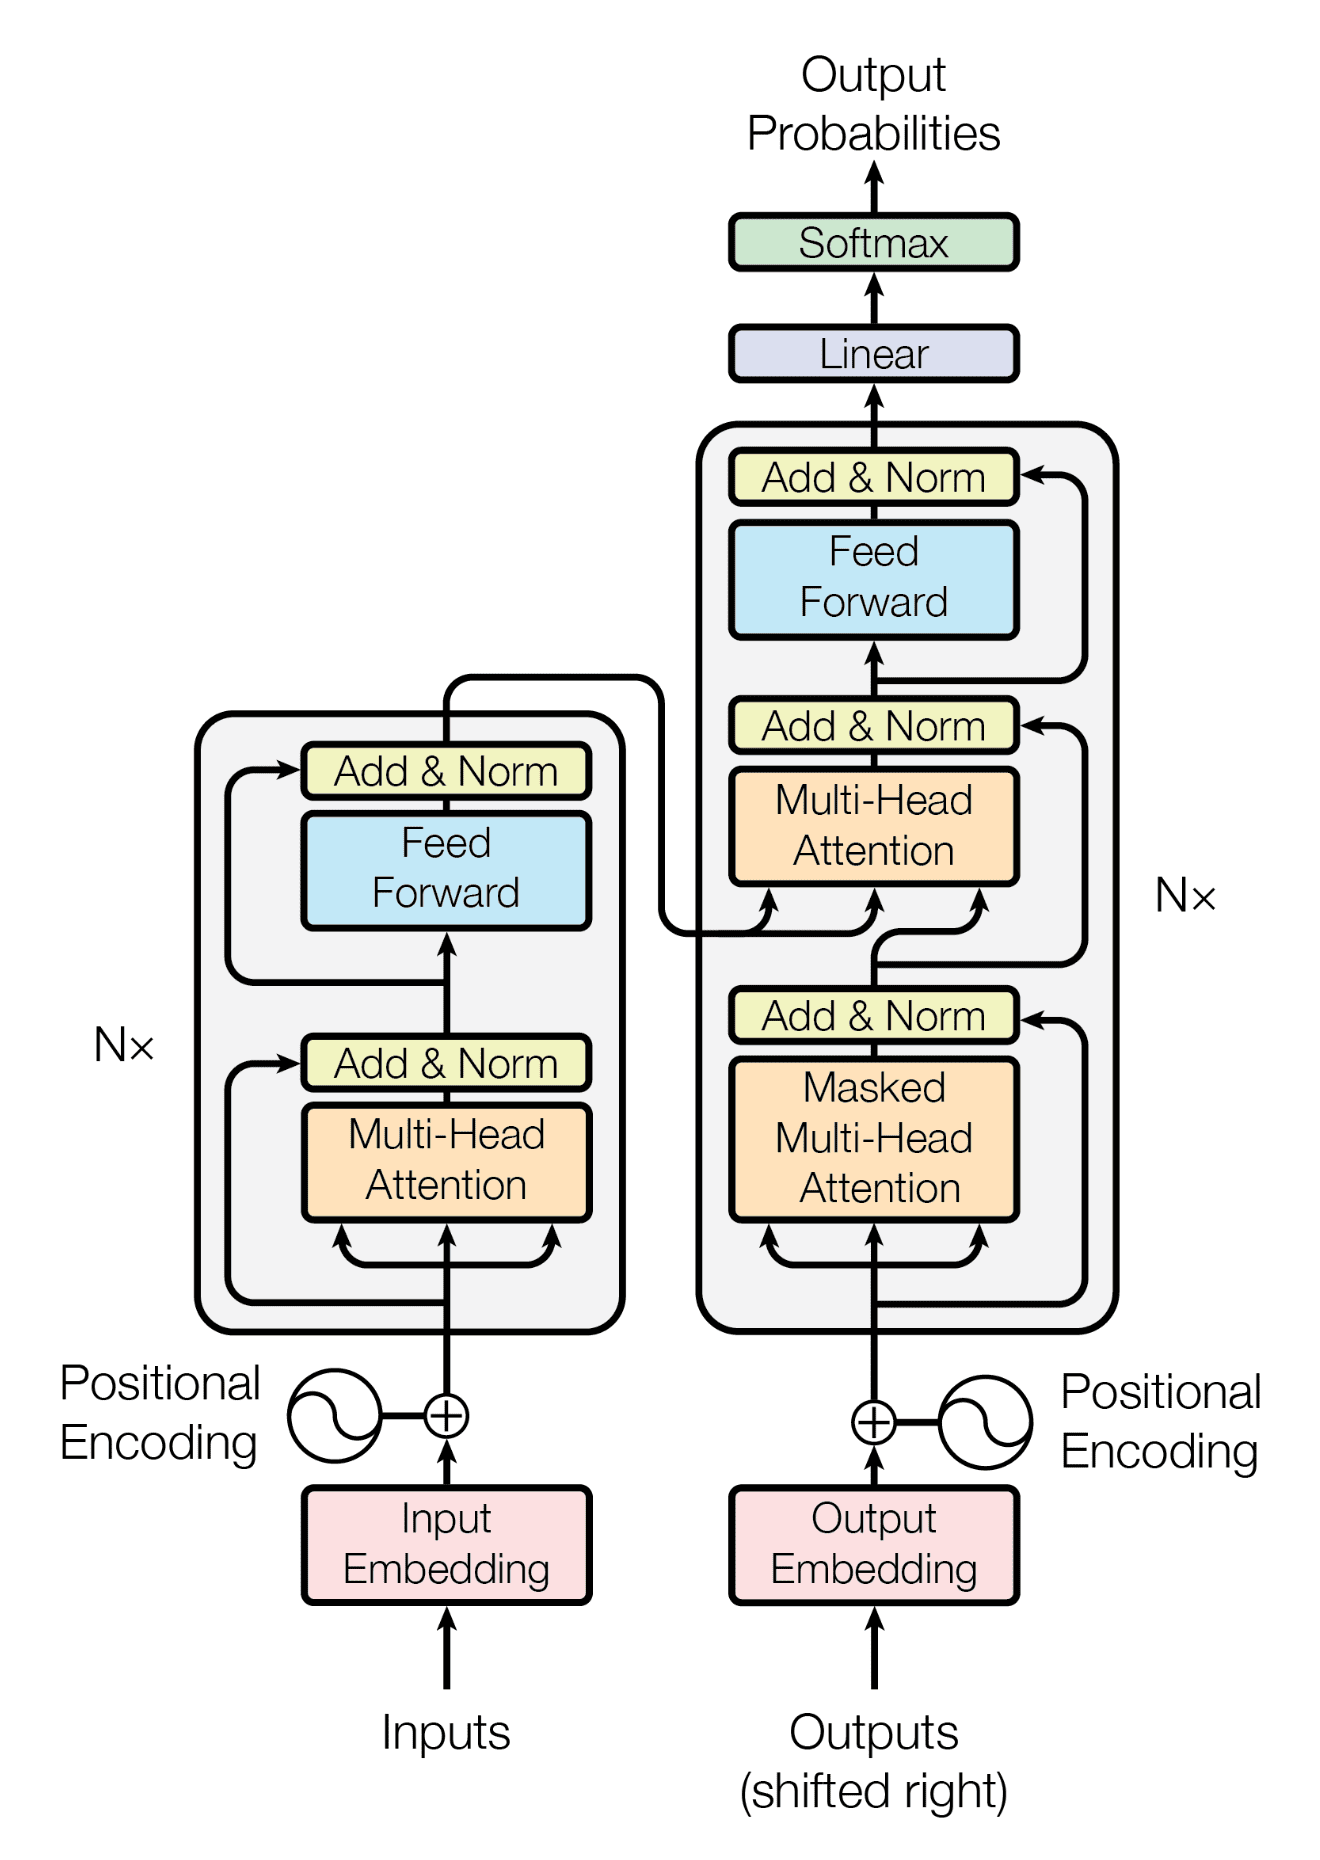
\includegraphics[width=6cm]{img/transformer.png}
  \caption{Architecture of the Transformer model.}
  \label{fig:transformer}
\end{figure}
The Transformer model, introduced in the influential paper "Attention is All You Need" by Vaswani et al. in 2017, represents a significant breakthrough in deep learning models. It emerged as a solution to tackle sequence-to-sequence tasks, with machine translation as its primary application. Prior to the Transformer's introduction, recurrent neural networks (RNNs) such as LSTMs dominated the field of sequence modeling and transduction. However, these RNN-based models posed challenges due to their sequential nature, which hindered efficient parallelization. As sequence length increases, the sequential computations of RNNs become a bottleneck. This limitation prompted the need for a more parallelizable approach. The Transformer architecture effectively addresses this parallelization problem by leveraging a novel technique known as self-attention. Self-attention enables the Transformer model to process sequences in a highly parallelized manner. Unlike RNNs, which depend on the sequential processing of each time step, self-attention allows for simultaneous computation across the entire sequence. This breakthrough concept revolutionized the field by efficiently capturing dependencies between different positions in the sequence. /cite{transformer} Today the Transformer has transcended its initial application in machine translation and has found utility across a wide range of domains. It is extensively employed in various areas of deep learning and natural language processing (NLP). /cite{transformersurvey}

In the following sections, we will delve into the basic architecture of the Transformer model and explore the intricacies of the self-attention mechanism.

\subsection{Self-Attention}
As can be seen in Fig. \ref{fig:transformer}, the Transformer consists of an encoder (left block) and a decoder (right block). As the BERT model only uses the encoder-part, we will only look at the inner workings of the encoder in this thesis. We will start with the Self-Attention mechanism inside of it.
Self-attention is a fundamental component of the Transformer model. It allows the model to capture relationships between different positions in a sequence. A concrete example of such a sequence is a sentence. Before computing the self-attention, the words within the sentence are transformed into vectors through an embedding algorithm. Consequently, each word is represented by a vector, forming a sequence of vectors. After that, positional encoding is applied to each input embedding vector by adding a positional encoding vector. These vectors represent specific positions in the input sequence, allowing the model to understand the order of the input data and capture sequential relationships. By incorporating positional encoding, the model can effectively process and interpret the words based on their position in the sentence.

Within the initial encoder, the sequence of vectors undergoes processing through two consecutive layers: the self-attention layer and the feed-forward layer. In the self-attention layer, each vector is split into three distinct vectors: a query-vector (Q), a key-vector (K), and a value-vector (V). These vectors are obtained by multiplying the input vector with three learned matrices, with each matrix dedicated to generating one of the respective vectors. These matrices are trained by the model during the learning process.

As a result, for each word in the sequence, we obtain three corresponding vectors: Q, K, and V. To compute the self-attention for a specific word, the dot product between its query-vector (Q) and the key-vectors (K) of all other words is calculated. This dot product operation produces similarity scores, representing the degree of similarity or relevance between the word and other words in the sequence.

To stabilize the gradients and ensure effective learning, the similarity scores are scaled. Additionally, a softmax function is applied to these scaled scores to normalize them. The softmax operation produces weights that indicate the relative influence or importance of each word on the word for which the self-attention is being computed.

Each value-vector (V) is then multiplied by its corresponding softmax-weight, and the resulting values are summed up. This aggregation process generates a new vector for the word under consideration. The new vector computed through self-attention encapsulates the original word's representation while incorporating the contextual information from the other words in the sentence. This integration of context within the new vector therefore captures the interdependencies and relationships among the words.

This process is done for all words in the sentence.

\subsection{Multi-Head Self-Attention}
Instead of generating a single attention vector for each input embedding, the original Transformer model utilizes a technique known as multi-head self-attention, where multiple attention vectors are computed simultaneously. Typically, eight attention vectors are calculated in parallel.

To accomplish this, the model employs multiple sets of Q, V, and K matrices, with the exact number determined by the number of attention heads used. Each input word embedding undergoes the self-attention process multiple times, with each iteration utilizing a distinct set of Q, V, and K matrices.

As a result, each word embedding in the sequence is associated with multiple attention vectors. To integrate the information from these attention vectors, they are concatenated together. The concatenated vector is then passed through the subsequent neural network layer, which follows the multi-head self-attention layer. 
One reason for the use of multiple attention heads is that the multiple attention heads allow the model to focus on different aspects of the input sequence. Thus the model can capture various patterns, relationships and dependencies among the data. This allows for a more comprehensive representation of the input, enabling the model to learn more nuanced and detailed information. 

\section{BERT}
\begin{figure} % add sections to this like in img/bert_overview.png
  \centering
  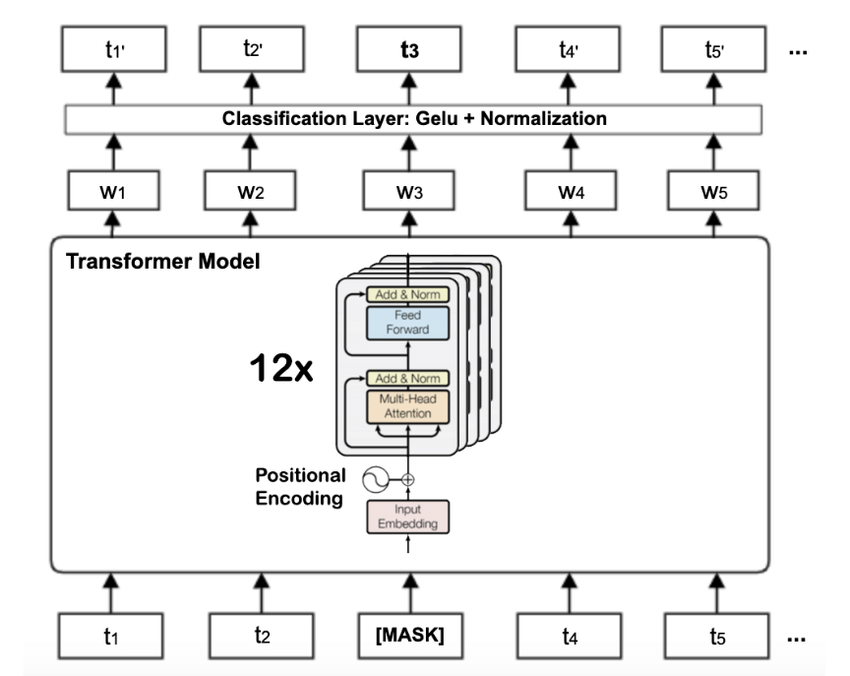
\includegraphics[width=12cm]{img/bert_architecture.png}
  \caption{Architecture of the BERT model.}
  \label{fig:bert_architecture}
\end{figure}
Having gained familiarity with the encoder part of the Transformer model, we now turn our attention to a powerful application of this architecture. In this section, we delve into the inner workings of BERT (Bidirectional Encoder Representations from Transformers), a system that leverages a multi-layer bidirectional transformer encoder. BERT builds upon the foundation laid by the original implementation of the Transformer to tackle complex natural language processing tasks. By exploring the intricacies of BERT, we aim to uncover the underlying mechanisms that contribute to its impressive performance in various language-related challenges.

\subsection{Background and Motivation}
The development of the BERT (Bidirectional Encoder Representations from Transformers) model was motivated by the need to overcome limitations of existing language models at the time. In this section, we will explore why BERT was developed and what differentiates it from other models.

At the time of BERT's introduction, standard language models predominantly utilized unidirectional encoders. These encoders processed input text in a sequential manner, either from left to right or right to left. However, the authors of BERT identified several disadvantages with this unidirectional approach.

Unidirectional encoders, by processing text sequentially, only have access to the preceding context at each position. This limitation poses a challenge in capturing dependencies that require information from both past and future tokens. For tasks that involve sentence-level understanding, such as question answering, incorporating context from both directions becomes crucial.

To address this limitation, BERT adopts a bidirectional approach. By leveraging a bidirectional transformer encoder, BERT processes input text in both directions simultaneously. This enables each token to access both preceding and succeeding context, facilitating a more comprehensive understanding of the context and capturing a wider range of dependencies. This makes it well-suited for various natural language processing tasks.


\subsection{Architecture and Inner Workings}
We will now delve into a detailed exploration of the architecture of the BERT model. Before we venture into the neural network aspect, it is crucial to understand the initial tokenization step employed by BERT.

\subsubsection{Tokenization}
\begin{figure}
  \centering
  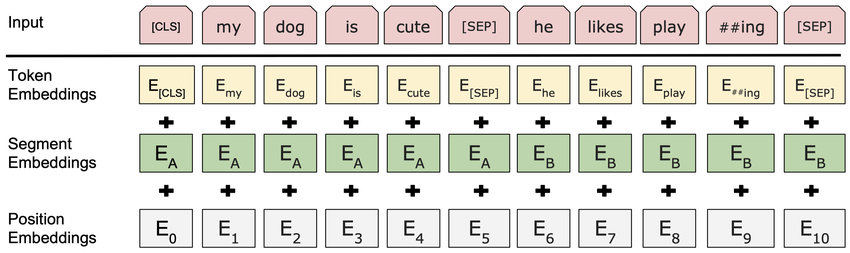
\includegraphics[width=12cm]{img/bert_input_representation.png}
  \caption{BERT input representation.}
  \label{fig:bert_architecture}
\end{figure}
The input to BERT consists of a string that can encompass multiple sentences. This string is initially divided into its constituent words. These words undergo embedding using the WordPiece model /cite{wordpiece}, where each word is mapped to a predefined vector representation.

In cases where the input contains words that are not present in the vocabulary, which consists of 30,000 tokens, these words are further divided into subwords that do exist in the vocabulary. For instance, if the word "playing" is absent from the vocabulary, it would be split into two words: "play" and "\#\#ing". The double pound symbol (\#\#) signifies that the subword is part of a larger word.

Within BERT's architecture, there are special tokens that play distinctive roles. Examples are the \textit{[CLS]} token, which indicates the start of a sequence, and the \textit{[SEP]} token, which denotes the separation between two sentences within the input.

After the string has been split up into tokens, which are limited to a maximum of 512 tokens in BERT, all tokens extracted from the input sentence are mapped to vector representations known as token embeddings. This token embedding captures the semantic meaning of each token within the sentence. Additionally, a segment embedding is added to the token embeddings. Together with the [SEP] token, these segment embeddings assist the model in discerning which sentence each word belongs to.

To incorporate positional information, a position embedding is added to each token embedding, indicating the token's position within the sequence. This positional encoding enables the model to consider the sequential arrangement of the tokens, similar to what we have observed in the Transformer model.

Upon completing these steps, we obtain the input embeddings, which are constructed by summing the token embeddings, segment embeddings, and position embeddings. These embeddings serve as the foundation for subsequent processing and comprehension by the BERT model. It is important to clarify that these embeddings themselves do not inherently contain contextual information yet. The responsibility of incorporating context lies with the self-attention mechanism within the neural network component of the model, which we are going to look at next.

\subsubsection{Neural Network Architecture}
BERT, as mentioned earlier, is a multi-layer bidirectional transformer encoder that builds upon the original transformer implementation, sharing many similarities. In the context of BERT, two versions were released: $\mathbf{BERT_{BASE}}$ and $\mathbf{BERT_{LARGE}}$. From here on we will only focus on the smaller $\mathbf{BERT_{BASE}}$ model, as in the classifier implementation we also use a smaller version of the model.

BERT is composed of 12 transformer encoders, stacked on top of each other, whereas the original transformer model had only 6. This increased depth is clearly illustrated in Figure 4. Within each encoder, there are 12 attention heads, surpassing the 8 used in the transformer model. Following the attention heads, there is a feed-forward layer, which in BERT has double the hidden size compared to the transformer.

Each encoder in BERT processes input and produces output vectors with a combined size of 768 elements. Consequently, BERT operates with a hidden size of 768 units. Impressively, BERT consists of a total of 110 million parameters, showcasing its capacity and complexity.


\subsection{Pre-training}
In this section, we dive into the pre-training phase of BERT by which the model is trained to comprehend language. This involves exploring the tasks it is trained on and the data utilized in the training process. Specifically, BERT undergoes training on two key tasks: Masked Language Modeling (MLM) and Next Sentence Prediction (NSP). In this section, we will begin by delving into the MLM task, which focuses on predicting masked words within a given context.

\subsubsection{Masked Language Modeling}
\begin{figure}
  \centering
  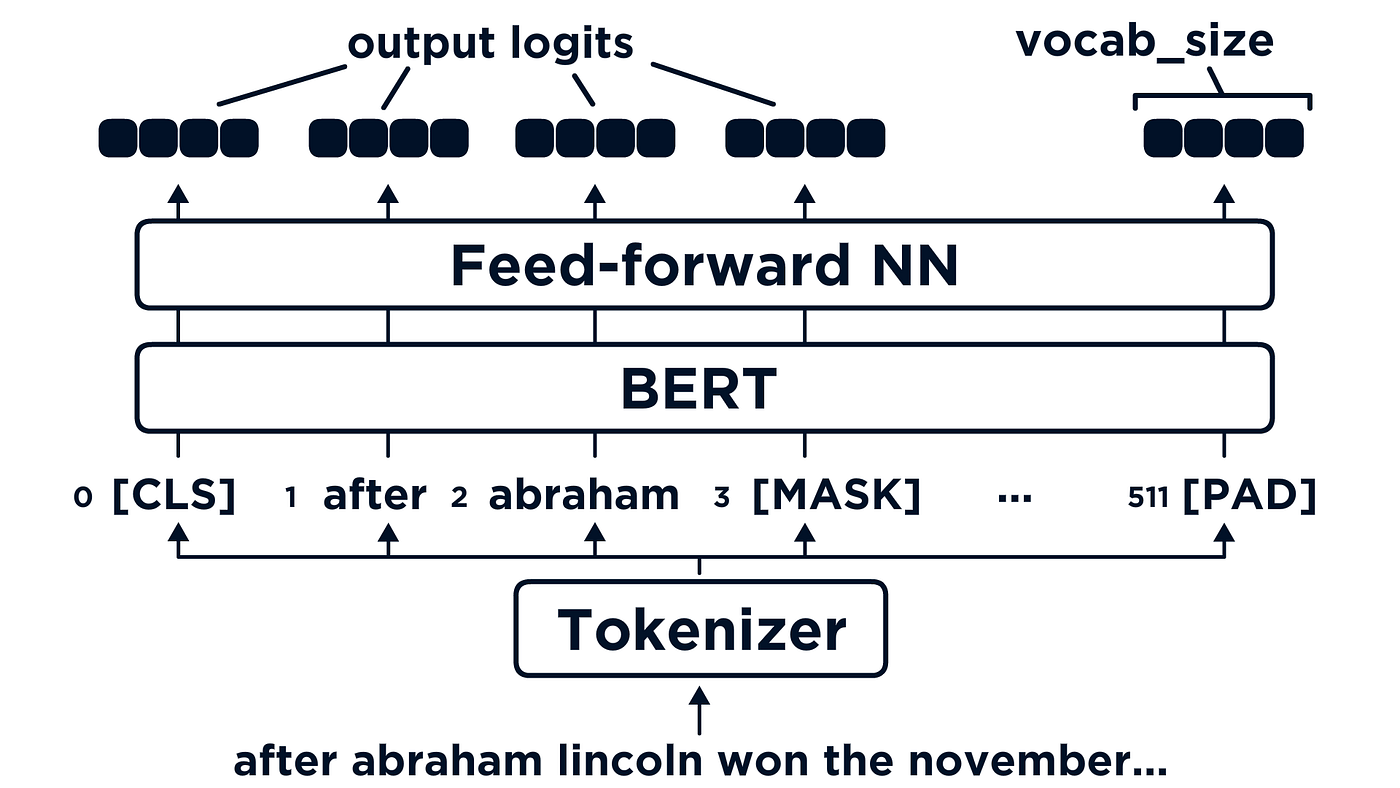
\includegraphics[width=12cm]{img/mlm_bert.png} % https://www.google.com/url?sa=i&url=https%3A%2F%2Ftowardsdatascience.com%2Fmasked-language-modelling-with-bert-7d49793e5d2c&psig=AOvVaw3N7c7ld6Z_BtHs7ImxP3TX&ust=1685946334954000&source=images&cd=vfe&ved=0CBEQjRxqFwoTCNC_4979qP8CFQAAAAAdAAAAABAs
  \caption{Masked Language Modeling in BERT.}
  \label{fig:mlm_bert}
\end{figure}
In the Masked Language Modeling (MLM) task, a crucial component of BERT's pre-training, approximately 15\% of the input tokens are randomly replaced with a special mask token, \textit{[MASK]}. This prompts the network to discern the most suitable replacement for the masked token. To achieve this, a feed-forward neural network is appended to each output of the last encoder layer.

These additional feed-forward layers include an output layer encompassing all English words. The outputs of these layers are then passed through a softmax activation function, resulting in a probability distribution across all English words. The word with the highest probability becomes the substitute for the masked token, enabling the model to predict the missing word.

This process allows the model to be trained bidirectionally, leveraging the entire context of the sentence, including words both to the left and right of the masked token. Consequently, the model develops contextual understanding, capturing the interdependencies between words.

However, an important consideration arises: the model could potentially learn to excel only in embedding masked tokens, which may hinder its performance when fine-tuned for different tasks lacking masked words. To address this, a small percentage of the chosen words for masking undergo various treatments:

\begin{itemize}
  \item 80\% of the words are masked with the \textit{[MASK]} token.
  \item 10\% of the words are substituted with random words.
  \item The remaining 10\% of the words remain unchanged.
\end{itemize}

By incorporating these variations, the model is compelled to maintain robust embeddings for all tokens. This helps mitigate potential performance degradation when fine-tuning BERT for different downstream tasks.

\subsubsection{Next Sentence Prediction}
During the pre-training phase, the model undergoes another procedure that enables it to understand the relationship between sentences. This procedure is formulated as a binary classification problem. Randomly selected sentences (referred to as A and B) are chosen from the corpus. In half of the instances, sentence B genuinely follows sentence A, while in the remaining cases, this sequential relationship does not hold. The model utilizes the output of the \textit{[CLS]} token as the binary classification output for this task.

\subsubsection{Pretraining Data}
The data used for pretraining the model consists of two major sources: the BooksCorpus and the English Wikipedia. These vast text collections provide a rich and diverse range of linguistic content for the model to learn from. The BooksCorpus dataset encompasses a substantial 800 million words, while the English Wikipedia dataset offers an even larger volume of 2,500 million words. 

By training on such extensive and varied textual data, the model gains a comprehensive understanding of the intricacies of language and can effectively leverage this knowledge in subsequent tasks.

\subsection{Fine-tuning}
The pretrained BERT model offers the flexibility to be fine-tuned for a wide range of tasks. To accomplish this, the outputs of the pretrained model are passed through a relatively simpler network that specializes in finetuning the model for a specific task. By adjusting the weights of this new network during the fine-tuning process, BERT becomes specifically tuned for the desired task. Compared to the pre-training procedure, where the entire model is trained from scratch, this fine-tuning process is significantly simpler and faster.

This streamlined approach of adjusting the weights of the added task-specific network makes BERT an attractive choice for tackling various NLP problems. It allows practitioners to adapt the powerful pretrained BERT model to their specific tasks, reducing the need for extensive training time and computational resources.


\subsection{Evaluation and Performance}
\begin{figure}
  \centering
  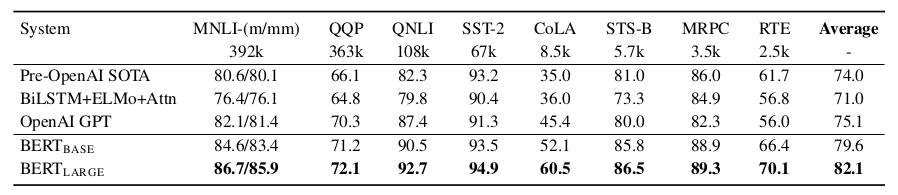
\includegraphics[width=12cm]{img/bert_results.png}
  \caption{GLUE Test results for BERT.}
  \label{fig:bert_results}
\end{figure}

The performance of BERT was evaluated through experiments conducted on the GLUE benchmark, which encompasses a diverse set of NLP tasks. In these experiments, the hidden vector corresponding to the \textit{[CLS]} token served as an aggregate representation. This representation was then passed through a classification layer for task-specific predictions.

BERT demonstrated impressive results across all evaluated tasks. Its performance was compared to prior state-of-the-art systems such as OpenAI GPT and ELMo. Notably, BERT consistently outperformed these systems, achieving superior accuracy and outperforming them by a significant margin.

It is worth mentioning that $\mathbf{BERT_{LARGE}}$ consistently exhibited better performance than $\mathbf{BERT_{BASE}}$, particularly when dealing with limited training data.

The results obtained from these experiments emphasize the superior performance of BERT across a wide range of NLP tasks. Additionally, they underscore the advantages of fine-tuning the model for specific applications, showcasing BERT's adaptability and effectiveness in various real-world scenarios.

\section{RoBERTa: Robustly Optimized BERT Pretraining Approach}
In 2019, a team at Facebook AI Research conducted a replication study of the BERT model. During this study, they developed an enhanced version of BERT known as RoBERTa. The name stands for Robustly Optimized BERT Pretraining Approach.

RoBERTa surpasses the performance of the original BERT model and achieves state-of-the-art results in various natural language processing tasks. In the following sections, we will explore the different design choices that were implemented in RoBERTa, comparing them to the original BERT model. This examination will provide insights into the advancements and improvements made in RoBERTa's architecture.

\subsection{Pre-training}
The primary distinction between RoBERTa and BERT lies in their pre-training approaches. Although the network architecture remains unchanged, the RoBERTa team conducted experiments with various variations of the MLM and NSP procedures and also tokenization. These variations were aimed at further improving the model's language understanding capabilities.

\subsubsection{Dynamic Masked Language Modeling}
In the original BERT model, masked language modeling (MLM) is performed in a static manner. This means that the masking of tokens is done once during the preprocessing stage. However, a limitation of this approach is that during training, the network would encounter the same masked training sequences multiple times as they are fed into it unchanged at each epoch.

To address this issue, the original BERT model duplicates each training instance ten times and applies a different mask to each duplicate. This technique ensures that the model sees variations of the masked training sequence. However, even with this approach, each training sequence is still observed four times with the same mask over the course of 40 epochs.

To overcome this limitation, RoBERTa introduces dynamic masking. With dynamic masking, a new masking pattern is generated every time a sequence is fed into the model. This approach is crucial when training the model for a larger number of epochs or with a larger dataset. Comparatively, the dynamic masking approach used in RoBERTa is comparable or slightly better than the static masking approach employed in the original BERT model.

\subsubsection{Necessity of Next Sentence Prediction}
Next Sentence Prediction (NSP) has played a significant role in the original BERT model's training process. It was initially deemed crucial for achieving high performance. The RoBERTa team however, arrives at a different conclusion regarding the necessity of incorporating the NSP loss.

Four different training formats were experimented with, and the findings suggest that the best-performing formats are the ones where NSP is not performed. Instead, sentences are sampled contiguously from a document until the maximum input size of 512 tokens is reached and then MLM is performed without the NSP task.

\subsubsection{Effect of Batch Size on Model Performance}
The study also investigated the impact of different batch sizes and learning rates on the performance of the model. This investigation was motivated by previous research, such as the work by Ott et al. (2018), which demonstrated the potential benefits of using larger batch sizes in for Neural Machine Translation.

The original BERT model was trained with a batch size of 256 and 1 million steps. The researchers wanted to explore the effects of different batch sizes while keeping the computational cost the same. By measuring the model's performance under various batch size configurations and adjusting the number of steps accordingly, they aimed to identify the optimal setup.

After conducting experiments on three different configurations, the study concluded that a batch size of 2k, a learning rate of 7e-4, and 125k steps produced the best outcomes. This configuration not only improved the model's performance on the given tasks but also offered the advantage of increased parallelizability, allowing for more efficient training.

\subsubsection{Larger Byte-level Byte-Pair Encoding}
\textit{\textbf{TODO}}

\subsubsection{Expansion of Pretraining Data}
In addition to modifying the pretraining tasks and hyperparameters, the training data was expanded significantly for the RoBERTa model.

In addition to the BookCorpus and English Wikipedia corpora, which together amounted to 16GB of text, several other datasets were included. These datasets included the \textit{CC-NEWS} dataset, comprising 63 million English news articles with a total size of 76GB, the \textit{OPENWEBTEXT} dataset consisting of content from various websites, totaling 36GB, and the \textit{STORIES} dataset, totaling 31GB. The incorporation of these additional datasets resulted in a combined training corpus size of 160GB.

By expanding the pretraining data to include a larger variety of text sources, the RoBERTa model was exposed to a more extensive and diverse range of linguistic patterns and structures.

\subsection{Evaluation and Performance}
\begin{figure}
  \centering
  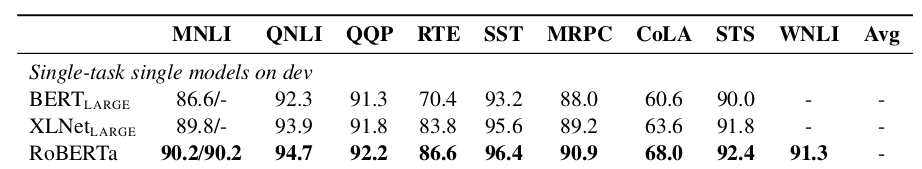
\includegraphics[width=12cm]{img/roberta_results.png}
  \caption{GLUE Test results for RoBERTa.}
  \label{fig:roberta_results}
\end{figure}
The performance of the RoBERTa model was assessed using various metrics and comparisons with other state-of-the-art models for different natural language processing tasks.

It was determined that the best performing configuration of RoBERTa utilized a training data corpus of 160GB, a batch size of 8k, and a total of 500K training steps. This configuration resulted in superior performance compared to other models. It significantly outpermorms the original $\mathbf{BERT_{LARGE}}$ model and also outperforms the $\mathbf{XLNet_{LARGE}}$ model across a range of NLP tasks.

An interesting observation made by the authors was that even the longest-trained RoBERTa model did not exhibit overfitting. This finding suggests that the model could potentially benefit from additional training, indicating the potential for further performance improvements.

The superior performance of RoBERTa in various language tasks, proves its effectiveness as a powerful language model. and the evaluation results confirmed the efficacy of the modifications and strategies employed in RoBERTa's training, leading to improved language understanding and representation capabilities.

\section{DistilRoBERTa} % distilbert
With the aim of harnessing the properties and advantages of the RoBERTa model, we have chosen it as the fundamental architecture for our classifier. RoBERTa however is, as we've just seen, a very big model with lots of parameters, which makes it somewhat slow compared to smaller models. This poses a problem for our use case, as our ultimate objective is to develop an interactive website that can deliver results to users quickly and efficiently. Therefore, it is crucial for our classifier to perform inference rapidly.

To achieve this goal, it was decided to utilize the DistilRoBERTa model provided by Hugging Face. DistilRoBERTa is a compressed version of the original RoBERTa model that maintains high performance while significantly reducing its size. This compressed model allows us to strike a balance between resource efficiency and accuracy.

Before delving into the details of our fine-tuning architecture, let us briefly explore the concept of knowledge distillation. Understanding how distillation works is key to appreciating how DistilRoBERTa has achieved remarkable compression.

\subsection{Knowledge Distillation} % distilbert, and the two papers on its page 2 under knowledge distillation
Knowledge distillation is a compression technique designed to enable a smaller model, referred to as the student, to replicate the performance of a larger model, known as the teacher. This process involves incorporating the teacher's predicted output distribution into the training of the student model. This is achieved through the use of a distillation loss in addition to the standard supervised training loss.

The intuition behind employing this distillation loss lies in the insight that the teacher's output distribution provides more informative signals to the student than the one-hot-encoded training distribution alone. By leveraging the teacher's knowledge and understanding, the student model can learn more effectively and capture the nuances present in the teacher's predictions.

\subsection{DistilRoBERTa Specifications} % distilbert
DistilRoBERTa, as indicated by its name, incorporates the knowledge distillation process to distill the knowledge from RoBERTa. In addition, it introduces several modifications to the RoBERTa model. These modifications include the removal of certain tokenization steps, a reduction in the number of layers, and the utilization of optimized linear algebra frameworks for linear layers and layer normalization.

These modifications have been remarkably successful, as demonstrated by the results. DistilRoBERTa achieves an impressive 95\% of the performance of RoBERTa-base on the General Language Understanding Evaluation (GLUE) benchmark. Notably, DistilRoBERTa also boasts significant advantages in terms of efficiency. It achieves twice the inference speed while being 35\% smaller in size compared to RoBERTa-base. 

This exceptional balance between performance and efficiency makes DistilRoBERTa a desirable choice for our use case.

\section{Finetuned DistilRoBERTa For Binary Future-related Sentence Classification}
\begin{figure}
  \centering
  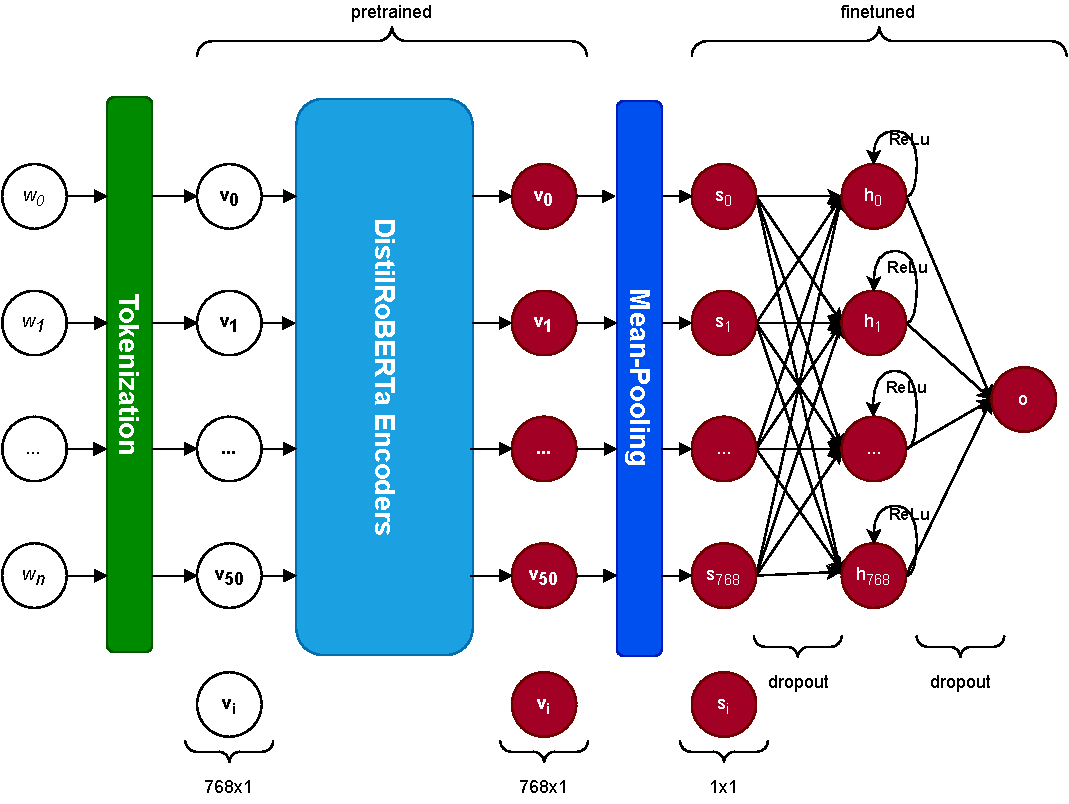
\includegraphics[width=15cm]{img/classifier_archi.pdf}
  \caption{Architecture of the classifier.}
  \label{fig:classifier_archi}
\end{figure}

In the figure provided, we can observe the high-level architecture of our classifier. In the subsequent sections, we will analyze the architecture's individual components, providing a detailed explanation and rationale behind the design choices.

\subsection{Optimized Tokenization for Reduced Complexity}
Firstly, from the figure it is evident that the number of tokens, also known as the sequence length, has been reduced to 50 tokens, thereby lowering the computational complexity and further increasing performance of the model. Considering that the model only processes one sentence at a time, and given that the average sentence length in our dataset is 20 words, this is sufficient.

\subsection{Mean-Pooling the DistilRoBERTa Outputs}
After the tokenization step, we obtain 50 embedding vectors, each having a dimension of 768. These vectors are then passed through the encoders of DistilRoBERTa. As a result, we obtain the same number of vectors with the same dimension, but now these vectors contain contextual information from the sentence. This contextual information, computed with attention, is visually represented by the red color in the figure.

While we now have contextualized embedding vectors for each input token, our goal is to classify the entire sentence as a whole. Therefore, it would be beneficial to have a single embedding vector that represents the entire sentence. This would also reduce the size of our finetuning feed-forward network. To achieve this, we compute the mean over all 50 embedding vectors. There are other ways to do this, such as utiliting the \textit{[CLS]} token, however HuggingFace recommends employing mean pooling. % /cite{https://huggingface.co/transformers/v4.7.0/model-doc/roberta.html}

Consequently, after the mean pooling operation, we obtain a single embedding vector of dimensionality 768. This vector captures the overall meaning and essence of the entire sentence, enabling us to perform efficient sentence-level classification on it next.

\subsection{Feed Forward Fine-Tuning Network}
The output of the mean-pooling operation serves as the input layer for our finetuning feed forward network. This network comprises a single hidden layer and a single output node, as we do binary classification. To introduce non-linearity, the hidden layer nodes are passed through a ReLU activation function. Additionally, dropout layers are incorporated before and after the hidden layer to mitigate overfitting and enhance generalization.


\subsubsection{Training Insights}
During the training phase, the weights of the finetuning network were initialized randomly. It is important to note that the weights of the pretrained model were frozen completely during the fine-tuning process, so they are not part of the training process. We employ the binary cross entropy with logits loss as our chosen loss function, which implicitly applies a sigmoid activation to the model output. The model was trained on our dataset over the course of 14 epochs with the following configurations: 
\begin{itemize}
  \item Batch size: 8
  \item Learning rate: $1.5e^{-6}$
  \item Warmup: 0.2
  \item Weight decay: 0.001
\end{itemize}
\begin{figure}[h]
  \begin{minipage}[b]{0.49\textwidth}
    \centering
    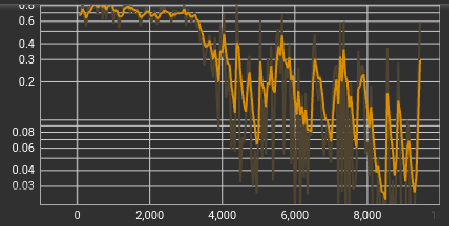
\includegraphics[width=\textwidth]{img/final_model_train_loss.png}
    \caption{Training Loss of the Final Model.}
    \label{fig:final_train_loss}
  \end{minipage}
  \hfill
  \begin{minipage}[b]{0.49\textwidth}
    \centering
    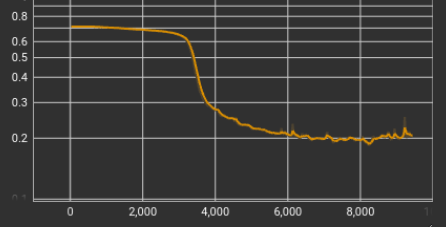
\includegraphics[width=\textwidth]{img/final_model_val_loss.png}
    \caption{Validation Loss of the Final Model.}
    \label{fig:final_valid_loss}
  \end{minipage}
\end{figure}

\subsubsection{Validation Insights}
We employed 10-fold cross-validation with early stopping to obtain performance estimates for the model. The training and validation losses for each fold are illustrated in Fig. \ref{fig:train_losses} and Fig. \ref{fig:valid_losses}, respectively. The following metrics show the average scores we achieved:
\begin{itemize}
  \item Accuracy: 0.965
  \item Precision: 0.953
  \item Recall: 0.98
  \item F1-score: 0.97
  \item AUC-ROC: 0.964
\end{itemize}

\begin{figure}[h]
  \begin{minipage}[b]{0.49\textwidth}
    \centering
    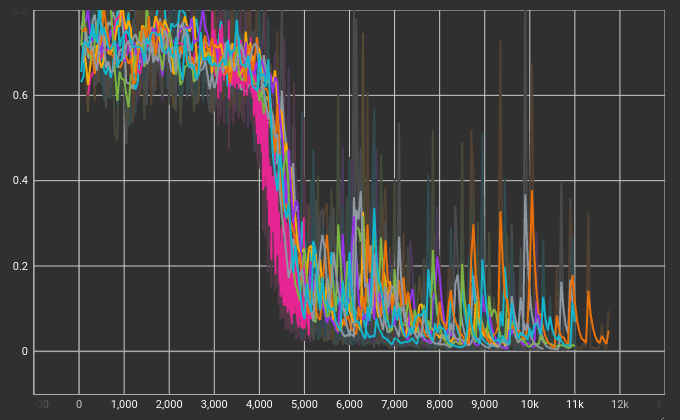
\includegraphics[width=\textwidth]{img/train_losses.png}
    \caption{Training Losses of the 10 fold cross-validation process.}
    \label{fig:train_losses}
  \end{minipage}
  \hfill
  \begin{minipage}[b]{0.49\textwidth}
    \centering
    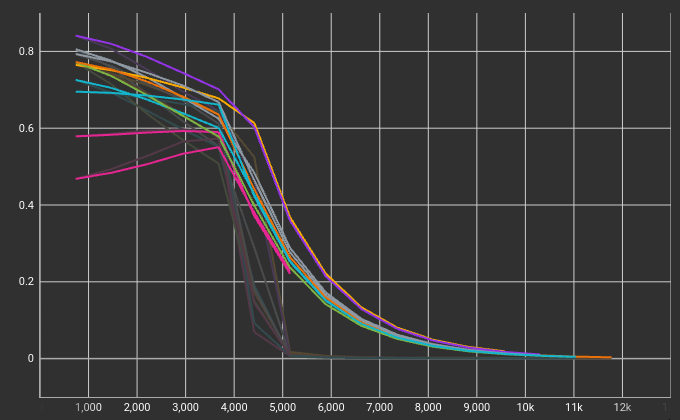
\includegraphics[width=\textwidth]{img/valid_losses.png}
    \caption{Validation Losses of the 10 fold cross-validation process.}
    \label{fig:valid_losses}
  \end{minipage}
\end{figure}

\subsubsection{Inference}
The prediction process involves the classification of sentences extracted from news articles into either future-related or non-future-related sentences.
First, all sentences extracted from news articles are subjected to classification using the trained model. The model assigns a confidence score between 0 and 1 to each sentence, indicating the likelihood of it containing future-related content. These confidence scores are then stored and analyzed.

Next, only sentences with a confidence score equal to or above 0.9 are considered as future-related sentences. They are then forwarded to the topic modeling component for further processing.

For sentences with confidence scores below 0.9, they are classified as non-future sentences. These sentences are stored in a separate database table. They can be later reviewed and manually inspected. Depending on the analysis, they may be added to the training dataset for further improvement of the model.
Also the future-related sentences are stored in the database and may be later added to the training dataset.

\subsection{Implementation}
The implementation of the DistilRoBERTa model with the appended finetuning network was done using PyTorch Lightning. PyTorch Lightning provided a simplified training process by reducing the amount of boilerplate code required for tasks such as data loading and model training.

\chapter{Topic Modeling}
In this chapter, we delve into the concept of topic modeling, a powerful technique that allows us to gain valuable insights from textual data. By leveraging topic modeling, we aim to enhance the user's understanding and exploration of future-related sentences within a given set of articles.

After downloading articles and classifying their sentences as future-related or not, the future-related sentences should be shown to the user. However, simply presenting these sentences individually may not provide a comprehensive understanding of the data. To address this, we explore the idea of grouping sentences together based on a specific criterion.

Among the various grouping strategies, organizing sentences by topic emerges as the most logical choice. By clustering sentences that share common content, we can present coherent and interconnected information to the user. This approach allows users to quickly gain an overview of the potential areas in which the requested entity holds future prospects.

So the primary objective of this chapter is to cluster sentences according to their topics and subsequently identify the most relevant keywords that encapsulate each cluster.

\section{Shortcomings of Conventional Models}
In the field of topic modeling, conventional models have long relied on representing documents as a mere bag-of-words, employing techniques such as Latent Dirichlet Allocation (LDA). One of the primary limitations of those conventional models is their failure to capture the intricate semantic connections that exist between words. By treating a document as a collection of independent words, these models disregard the rich contextual information that can be derived from the interplay of words within a sentence or paragraph.

The rise of text embedding models revolutionized the way we understand and analyze textual data. Leveraging the success of these text embedding models, researchers began incorporating them into the realm of topic modeling.

One notable approach that bridges the gap between text embedding models and topic modeling is Top2Vec. Instead of relying solely on the traditional bag-of-words representation, Top2Vec adopts a more comprehensive strategy. It clusters document embeddings, which capture the semantic essence of the entire document, and extracts topic representations by identifying words whose embeddings closely align with the centroid of each cluster. These representative words effectively encapsulate the dominant theme or topic of the respective cluster.

However, it is important to acknowledge that even approaches like Top2Vec have their limitations. One key problem arises from the assumption that words near the cluster centers are the most representative of the topic. While this assumption holds true in many cases, clusters in real-world data often deviate from a spherical shape around their centers.

The misalignment between the assumption of spherical clusters and the actual distribution of data points can result in misleading topic representations as the words in close proximity to the cluster centroid may not accurately capture the full range of concepts and themes encompassed by the cluster. This limitation highlights the need for more advanced techniques that can accommodate complex cluster shapes and provide more accurate representations of topics within the data.

\section{BERTopic}
In the quest to address the limitations we have discussed, an innovative topic modeling approach called BERTopic has emerged. This methodology leverages clustering techniques and a class-based Term Frequency-Inverse Document Frequency (TF-IDF) to overcome the challenges posed by traditional models.

To accomplish its goal of effective topic modeling, BERTopic operates through a three-step process. In the following sections, we will delve into each step to gain an understanding of BERTopic's functionality.

\subsection{Document Embeddings}
The initial step involves mapping documents to a vector space, which can be accomplished through an embedding process. In the case of BERTopic, a pre-trained language model called SBERT is utilized for this purpose. As the name suggests, SBERT is based on BERT.

There is a significant distinction between BERT and SBERT in their respective embedding approaches. BERT focuses on generating word embeddings that capture the meaning and context of individual words within a sentence. It achieves this by considering the surrounding words and their relationships. /cite{bert} On the other hand, SBERT aims to map similar sentences to similar vectors in the embedding space, specifically using cosine similarity as a measure. /cite{sbert}

While BERT can also generate sentence embeddings by employing pooling techniques or the [CLS] token, studies have shown that this approach produces subpar results. /cite{sbert} In contrast, SBERT has achieved state-of-the-art performance on various sentence embedding tasks, making it the default choice for BERTopic. /cite{bertopic}

However, it is important to note that it is possible to replace SBERT with alternative models if desired. BERTopic allows flexibility in selecting different models for generating sentence embeddings, enabling customization based on specific requirements or preferences.

\subsection{Document Clustering}
In the task of document clustering, a challenge arises as the dimensionality of the data increases. At higher dimensions, the distance to the nearest point tends to approach the distance to the farthest point. Consequently, the concept of spatial locality becomes ambiguous, as the differences in distances become negligible.

This issue becomes problematic when attempting to cluster the high dimensional sentence embeddings generated in the previous step. One effective approach is to reduce the dimensionality of the embeddings before performing the clustering process.

A notable technique employed by BERTopic, is the utilization of a data dimensionality reduction algorithm called UMAP. This algorithm has demonstrated its ability to preserve both local and global features, providing a means to alleviate the challenges posed by high-dimensional data.

After applying the dimensionality reduction using UMAP, the reduced embeddings are ready for clustering. For this task, BERTopic employs the HDBSCAN algorithm. HDBSCAN is a robust clustering algorithm that is capable of identifying clusters of varying densities in the data, making it suitable for the clustering of document embeddings.

By employing these sequential steps of dimensionality reduction and subsequent clustering, BERTopic offers an effective solution for document clustering tasks.

\subsection{Topic Representation}
Now that the data is organized into clusters, the next step is to extract topic representations from these clusters. To achieve this, a modified version of the TF-IDF (term frequency-inverse document frequency) technique is employed, which measures the importance of words in a document.

Traditionally, TF-IDF considers the frequency of a term within a document and the number of documents that contain the term. However, in the modified approach, all documents belonging to the same cluster are combined into one document. This adjustment allows to capture the significance of words within clusters, rather than individual documents.

The inverse document frequency is then computed by taking the logarithm of the average number of words per cluster divided by the frequency of the term across all classes. To ensure a positive outcome, one is added to the computed result.

This modified approach makes it possible to model the importance of words within clusters. As a result, the most important words can be identified as representatives of each topic, facilitating a more precise understanding and representation of the topics at hand.

\subsection{Configuration of BERTopic for Future-related Sentence Clustering}
In this section, we will delve into the concrete configuration of BERTopic in our project and evaluate its performance on the news data.

In order to achieve optimal results, certain parameters of BERTopic were tailored and adjusted from their default values. The specific configuration used in this project is outlined below:

\begin{itemize}
    \item \textbf{Sentence Embedding Model:} To generate high-quality sentence embeddings, the "all-MiniLM-L6-v2" model from the SentenceTransformer library was chosen.

    \item \textbf{Vectorizer Model:} A CountVectorizer was utilized after the embedding process to remove stopwords from the text data. This step was implemented to exclude commonly occurring words that lack substantial semantic significance from the resulting topic representation.

    \item \textbf{Top Words per Topic:} BERTopic was configured to provide a concise summary of each topic by extracting the top 10 most representative words associated with each cluster.

    \item \textbf{Minimum Topic Size:} The minimum topic size was adjusted to five in order to address the issue of having excessively large topics containing multiple subtopics. By reducing the minimum topic size, the granularity of the topics was increased.

    \item \textbf{Dimensionality Reduction Model:} UMAP\footnote{\url{https://umap-learn.readthedocs.io/en/latest/}} was used for dimensionality reduction.

    \item \textbf{Clustering Model:} HDBSCAN\footnote{\url{https://hdbscan.readthedocs.io/en/latest/}} served as the clustering method.
\end{itemize}

\begin{figure}
  \centering
  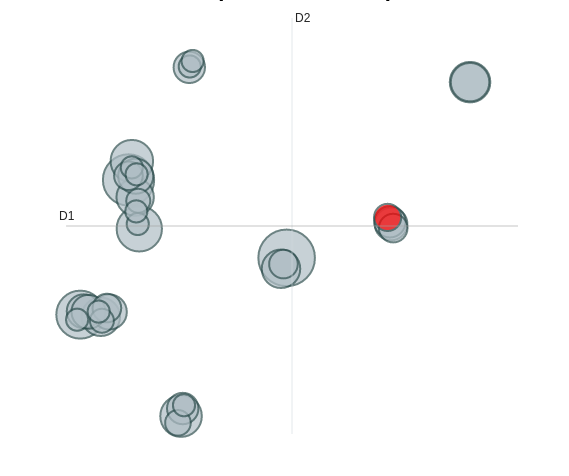
\includegraphics[width=10cm]{img/intertopic_distance_map.png}
  \caption{Intertopic Distance Map for Sentences from Ukraine-related News Articles using BERTopic.}
  \label{fig:intertopic_distance_map}
\end{figure}

\begin{figure}
  \centering
  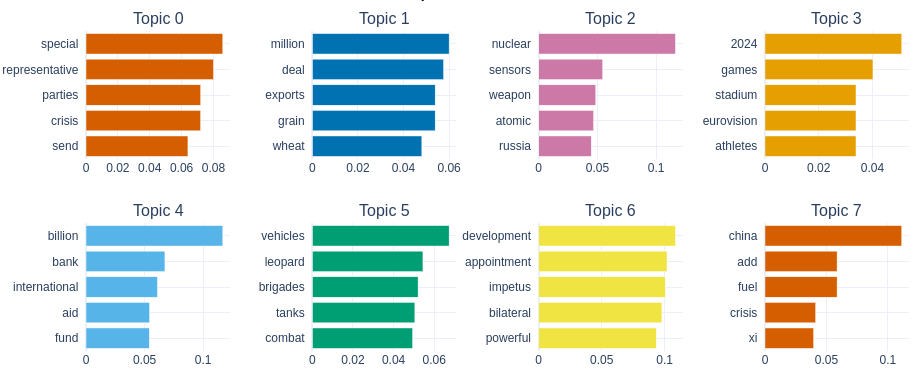
\includegraphics[width=15cm]{img/topic_representation.png}
  \caption{Topic Representation and c-TF-IDF Scores Generated by BERTopic.}
  \label{fig:topic_representation}
\end{figure}


\chapter{Temporal Expression Identification and Extraction}
An important objective of this work is to associate sentences related to the future with a coherent timeline. To achieve this, a crucial preliminary step involves dissecting sentences to identify any temporal expressions they contain. Once this temporal information is identified, it is extracted and mapped to a specific date. Then it is possible to map a sentence to a concrete point in time and therefore to a concrete point on a timeline.

\section{SUTime - Temporal Tagger}
A system designed for this specific task is referred to as a 'temporal tagger'. In this work, a rule-based temporal tagger named 'SUTime', integrated within the Stanford CoreNLP pipeline, serves as the central instrument. Despite its inception in 2012, SUTime continues to excel in its functionality, as demonstrated throughout this exploration.

\subsection{Inner Workings}
SUTime, the engine driving the temporal tagging process, employs a systematic approach structured around three stages:

\begin{enumerate}
  \item In the first stage, the system analyzes the the text to identify words that could potentially form numerical expressions.

  \item Having identified numerical expressions, the system can use those in addition to the other words to start looking for simple temporal expressions.

  \item In the final stage, basic temporal expressions are combined to create more complex expressions
\end{enumerate}

This strategy is implemented through different types of patterns that SUTime supports for matching text: token patterns, string patterns, and time patterns.

\begin{itemize}
  \item \textbf{Token patterns} operate over individual tokens in the text. A token is typically a word, number, punctuation or other meaningful unit of text. Token patterns in SUTime use a regular expression language (TOKEN-SREGEX) which is included in the Stanford CoreNLP package that works on tokens instead of raw text strings. This allows for the use of token annotations in the matching process. For example, a rule can be specified that matches a token like 'years' and maps it to a predefined duration type YEAR. More complex rules can then also be designed using macros or annotations that match specific types of tokens, such as numbers and duration units.

  \item \textbf{String patterns} operate at the string level, which means they consider the text as a whole and can match patterns anywhere in the text, regardless of token boundaries.

  \item \textbf{Time patterns}, on the other hand, are used for matching time-specific patterns over text that align with standard date/time formats.
\end{itemize}

Upon recognition of all temporal expressions, relative times are transformed into absolute references relative to the specified reference date. The results are returned in the form of TIMEX3 annotations, which is a standard to capture temporal information in natural language.

\subsection{Limitations}
The capabilities of SUTime are not without their limitations - points acknowledged by the system's creators. Although most of these constraints have little bearing on our specific use-cases, one stands out as particularly relevant.

While the tagger generally performs well, there are some problems with ambiguous references like ’On Tuesday, he revealed his decision, which will become official soon’. The time-tagger maps "on Tuesday" to the coming Tuesday, which is in the future, even though the sentence is referring to a past event. This is mitigated by simply discarding extracted temporal expressions that reference weekdays.

Given the recurrent occurrence of this issue during system testing, a decision was taken to exclude all temporal expressions referencing weekdays. This step was deemed necessary to ensure the system's accuracy and reliability in the face of this particular challenge.

\subsection{Comparative Analysis of SUTime Against Other Temporal Tagging Systems}
In order to evaluate the effectiveness of the SUTime temporal tagger, the authors conducted a series experiments comparing its performance against other contemporary state-of-the-art systems. The systems chosen for comparison were GUTime, HeidelTime, and TRIPS/TRIOS. These experiments aimed to shed light on the strengths and weaknesses of SUTime in the context of temporal expression identification.

The authors discovered that both rule-based systems, exemplified by HeidelTime, and probabilistic systems, represented by TRIPS/TRIOS, exhibited comparable effectiveness in recognizing temporal expressions. This equivalence was reflected in their similar F1 scores, highlighting that rule-based approaches could capture a significant portion of temporal patterns.

However, among the systems under examination, SUTime emerged as the frontrunner in terms of performance, achieving the highest F1 score and recall for identifying temporal expressions. This outcome underscores the proficiency of SUTime in accurately and comprehensively detecting temporal nuances within text.

It's worth noting that the absence of language models during the time of SUTime's release precluded their inclusion in this comparative analysis. Consequently, this study offers valuable insights into the effectiveness of SUTime relative to its contemporary temporal tagging systems.


\chapter{System Implementation and Architecture}
In this chapter, we will delve into the detailed implementation of the frontend and backend components of the web application, which can be accessed with a standard browser at the following URL: \url{http://chronicle2050.regevson.com}. We will explore the design choices made, the structure of the system, and the integration of various technologies and frameworks. This chapter highlights the development process, from the frontend user interface to the backend server architecture, ensuring a comprehensive understanding of the system's implementation.

\section{Frontend Implementation}
In this section, we will explore the various aspects of the frontend implementation for our web application. We will delve into the rationale behind the frontend framework selection, discuss the UI design and layout considerations, and examine specific features and functionalities implemented in the frontend.

\subsection{Frontend Framework Selection}
For this project, a frontend framework called Vue.js (Vue) was chosen. Vue is a powerful framework that uses HTML, CSS, and JavaScript to enable efficient development of user interfaces. It accomplishes this by providing support for two fundamental features:

\begin{itemize}
  \item \textbf{Declarative Rendering:} Vue extends standard HTML by introducing a template syntax that enables developers to embed JavaScript state directly into the HTML. This approach allows for more intuitive and concise UI development.

  \item \textbf{Reactivity:} One of Vues key strengths is its reactivity system. It monitors changes in the JavaScript state and automatically updates the Document Object Model (DOM) to reflect those changes. This feature eliminates the need for developers to manually manipulate the DOM, resulting in increased productivity and code maintainability. /cite{vuejs website}
\end{itemize}

While there are numerous frameworks on the market offering similar functionality, Vue stands out as one of the most popular choices alongside Angular and React. All these modern frontend frameworks have large communities, active maintenance, extensive documentation, and good performance. However, Vue possesses specific strengths that were particularly important for this project, ultimately leading to its selection as the frontend framework.

First and foremost, Vue is highly praised for its simplicity and gentle learning curve. Its intuitive syntax and straightforward concepts make it easier for developers to grasp and start building applications quickly. This aspect was important for this project, where the ability to swiftly get started and incorporate changes efficiently was crucial. On the other hand, Angular and React are often considered somewhat more heavyweight, difficult, and complex in nature. /cite{frontend-frameworks}

So by choosing Vue, a simple and efficient development process was implemented, enabling the rapid creation of the desired user interface while maintaining a manageable codebase.

\subsection{UI Design and Layout}
In this section, we will delve into the planning and design of the user interface.

\subsubsection{Design Workflow}
Before implementing the HTML/CSS layout, the UI was initially conceptualized and designed using Photoshop. This workflow allowed for a quick visualization of the ideas before investing time into their actual implementation, which can be a more time-consuming process. %Figure XY showcases a comparison between a Photoshop draft and its final implementation.


\subsubsection{Settings and Input}
Upon entry, the website shows a settings panel that provides the user with some adjustable configurations. Here, decisions about whether updates should be automatic or manual can be made. There’s also the possibility to specify the quantity of articles and their time frame. A text field prompts users to specify an entity for exploration.

\subsubsection{Statistics}
The website also includes a dedicated statistics section to provide users with insightful information:

\textbf{Percentage of sentences with and without temporal expressions:} Users can identify the percentage of sentences that contain temporal references, such as "next year" or "this August." \\
\textbf{Number of clusters:} Users can obtain information about the total number of clusters present in the dataset. \\
\textbf{Average number of sentences per cluster:} This statistic showcases the average quantity of sentences that are associated with each cluster. \\
The presentation of these statistics is designed to provide users with a comprehensive overview and enhance their understanding of the returned data.

\subsubsection{Timeline Visualization}
 The timeline section is one of the key components of the website. It offers valuable insights into the relationships between topics and the referenced dates within the associated sentences.

\paragraph{Axes}
The y-axis of the timeline contains all topics that contain sentences with temporal expressions. As already mentioned those temporal expressions could be phrases like "next August", "this Summer", ... . The topics on the timeline are organized in a manner that reflects their relevance. This arrangement places more relevant topics towards the top of the y-axis, while less relevant ones are positioned towards the bottom. The specific criteria used to determine relevance will be explored and explained in detail in section XY.

On the other hand, the x-axis displays a continuous series of dates, signifying the future dates referred to by the temporal expressions within the sentences.

\paragraph{Datapoints}
To provide a concrete example: a data point on the timeline, with coordinates (x, y), represents a collection of sentences belonging to topic y. These sentences contain temporal expressions referencing the date x.

Hovering over or clicking on a data point on the timeline reveals a tooltip section containing all sentences associated with the topic and the referenced date. Each sentence is accompanied by a numerical count, indicating how often it is mentioned in the news corpus. To avoid duplicate content, similar sentences offering the same information are intelligently removed to avoid redundancy and also count as mentions. A brief notification informs users about the omitted sentences due to similarity.

Furthermore, the section offers an option to display sentences linked to the topic, even if they lack temporal expressions and do not appear on the timeline. This inclusiveness provides a more comprehensive view of the topic and its context. To get more information, clicking on a sentence opens a new tab displaying the entire article from which the sentence was extracted. This feature enables users to access the full context, gaining deeper insights and making well-informed interpretations.

\subsubsection{Word Cloud Visualization}
The Word Cloud showcases sentences that lack any temporal expressions and is positioned beneath the timeline.

Each distinct topic within the corpus receives its own dedicated cloud, displaying the most representative words associated with that topic. The size of each cloud dynamically adjusts based on the relevance of the corresponding topic, offering a visual cue about its significance.

Furthermore the Word Cloud is interactive. When users hover or click on a specific cloud, a tooltip emerges, revealing all the relevant sentences that belong to that particular topic. Just like with the timeline-tooltip, users can click on any sentence within the tooltip to instantly access its source article. Moreover, the number of times each sentence appears in the corpus is indicated next to it, providing additional context about its frequency and importance.

\subsubsection{Log Visualization}
To ensure that users are continuously informed about the backend processing progress, a Log View was introduced that can be easily toggled open or closed.

Within this Log Section, users can access important information about the ongoing processing. Here are the key details provided:

\begin{itemize}
  \item \textbf{Total Number of Articles Fetched:} This figure represents the entire count of articles that are retrieved from the internet.

  \item \textbf{Number of Fetched Articles:} Users can keep track of the precise number of articles that have already been fetched and processed.

  \item \textbf{Total Number of Updates:} This indicates the overall count of updates that are processed by the backend.

  \item \textbf{Number of Remaining Updates:} To give users a clear understanding of the remaining work, this metric highlights the number of updates yet to be processed by the system.
\end{itemize}

Towards the end of the log-view, all the log-messages from the backend are conveniently printed out. This enables users to gain an in-depth understanding of the system's activity and progress.

\subsubsection{Charting Library}
The timeline was brought to life using ApexCharts, a powerful charting library that facilitates the creation of vibrant and interactive visualizations for web pages. Being an open-source project, ApexCharts offers flexibility and versatility to developers. /cite{apexcharts}To seamlessly integrate ApexCharts with Vue.js, a library called vue3-apexcharts was utilized, which acts as a convenient wrapper library. This integration empowers Vue developers by allowing them to effortlessly incorporate and interact with ApexCharts using the familiar Vue syntax. /cite{vue3-apexcharts}

\subsection{Interaction with the Backend}
The frontend and backend work together seamlessly to provide a good experience to the user. When the user clicks the "Explore" button, Axios, a popular JavaScript library for handling HTTP requests, comes into play. It triggers an HTTP GET request towards the backend's 'start/' endpoint, prompting the backend to begin the retrieval, classification, clustering, and tagging processes.

As the backend processes the data, the frontend diligently polls the 'status'-endpoint, continuously receiving an array containing a checksum value and essential processing status information. This checksum value acts as a unique identifier for the current status of the database. Whenever a change occurs in the database, such as the availability of new sentences ready for presentation, the checksum value changes, prompting the frontend to visualize the new data on the timeline and word cloud.

Furthermore, the statistics are updated to reflect the most current information available. The response from the 'status'-endpoint also includes crucial details about the ongoing processing status on the backend for the requested entity. The frontend meticulously processes this information and keeps the log section up-to-date, providing users with a deeper understanding of the progress being made.



\section{Backend Implementation}
With a clear grasp of the layout and insight into the frontend-backend interaction, the focus now shifts to a comprehensive examination of backend implementation. Delving into the intricate workings of the backend will illuminate how this vital component is precisely realizeed.

\subsection{Django Framework}
The backend infrastructure was developed with the Django Framework. It is an open-source platform and is built upon the foundation of the Python programming language, leveraging Python's principles and capabilities. With its exceptional agility, Django empowers developers to swiftly translate their concepts into reality, ensuring rapid idea realization. One of its standout attributes lies in its scalability which allows developers to build applications that can handle increased user loads and growing datasets. While such features are present in many well-regarded frameworks, Django was chosen specifically due to its alignment with the Python programming language. As the classifier is implemented with pytorch in python, it was apparent to use a python-based framework like Django for the backend. Moreover, Django seamlessly integrates with a REST framework, making it very easy to create and expose endpoints. The framework's simplicity further contributed to its selection, making it an ideal choice to kickstart and swiftly implement various functionalities.

\subsection{Article Downloading Implementation}
The user initiates the process by specifying the desired number of articles for download, accompanied by a designated timeframe that dictates the acceptable publication dates. Then an HTTP request, containing the user's criteria, is dispatched to the newscatcher-server.

Following the data retrieval, irrelevant attributes are eliminated, leaving behind only the core elements of each article. These refined articles are stored in a newly created database table. This table stores details, such as article titles, content, publication timestamps, associated topics, and hyperlinks to the articles.

\subsection{Preprocessing Implementation}
In the preprocessing stage, the articles are initially downloaded in JSON format, containing various attributes such as title, excerpt, article, timestamp, topic, and link. However, only the relevant attributes including article, timestamp, topic, and link are stored in the database for further processing.

To ensure data quality, articles with an empty article field are removed from the dataset. Next, the Python NLTK library is employed to tokenize the remaining articles into sentences.

Following tokenization, the length of each sentence is calculated, and any sentences with a length below 30 are filtered out. This step helps to focus on sentences that provide substantial content and minimize noise in the dataset.

To address duplicate sentences, a deduplication process is applied. Duplicate sentences are removed, while keeping track of the count of duplicates for each sentence. This count becomes valuable in later stages for computing the relevance of individual sentences.

Finally, the processed sentences are stored back into the database, ensuring a clean and refined dataset ready for subsequent processing.

\subsection{Classification Implementation}
After the articles are split up into sentences and subjected to preprocessing, the classification step itself is executed. This process takes place remotely using Google Colab, due to its ability to offer high-speed GPU processing capabilities. This proves to be important for the web application's online inference requirement, demanding optimal speed.
Google Colab becomes even more appealing due to the availability of XYZ GPUs, enhancing performance without any associated costs. Yet, it's important to acknowledge a limitation - the webapp is only functional when the Colab notebook is running. Thus the accessibility of the service is restricted and can therefore only be used for demonstration and development purposes.
However, as time progresses, there is a potential to replace the Colab server with a web server that has fast GPUs and offers better availability.
The implementation of the DistilRoBERTa model, augmented with a finetuning network, was orchestrated using the efficiency of PyTorch Lightning. This framework simplified the training trajectory by minimizing redundant code, simplifying tasks like data loading and model training.
After classification, sentences that carry a model confidence level exceeding 0.8 are stored within a designated database table, ready for the subsequent clustering phase.

\subsection{Clustering Implementation}
The clustering step again takes place within the Google Colab environment, leveraging its powerful GPU capabilities for better speeds.

The clustering step is straightforward due to the simple nature of BERTopic. As detailed in Section XYZ, the specific parameter values that govern this phase have already been established. BERTopic generates an array for each topic, filled with sentences belonging to that topic, alongside a corresponding array housing the sentence embeddings for further analysis.

In the next step, representative keywords are extracted while simultaneously eliminating any stopwords.

Then a structured dataframe is assembled, capturing essential information for each sentence. One such piece of information is the number of representative keywords a sentence contains. For this, the top 6 keywords of the sentence's associated topic are considered and matched against the words in the sentence itself. Any sentence falling short of containing at least 3 of these keywords is pruned from the dataset. This process improves the alignment between the topic keywords and the retained sentences.

Next the cosine similarity between all sentence embeddings within the same topic is calculated. A threshold is set, with sentence pairs exhibiting a similarity above 0.8 being identified as duplicates. So every sentence gets assigned a count of its (exact and approximate) duplicates within the assigned topic.

The final stages of processing are dedicated to ensuring the integrity of the generated clusters. Sentences with a cosine similarity exceeding 0.7 are classified as similar. The sentence with a higher duplicate count is retained, while its counterpart is excluded. This ensures that clusters remain diverse and insightful, avoiding redundancy that might arise from differently formulated sentences discussing the same information.

The results of this process find their place in a dedicated database table. This table stores the processed sentences alongside their respective topics and duplicate counts. These sentences await the subsequent time-tagging process.

\subsection{Time Tagging Implementation}
The Time Tagging procedure involves the systematic extraction and classification of temporal expressions, known as TIMEX, from the clustered sentences.

To accomplish this, the SUTime parse function is employed. The workflow is structured as follows: first the sentences are retrieved from the database. These sentences are then passed to the SUTime parse function alongside their associated publishing date, yielding a JSON object as output. This object either contains the identified TIMEX along with its type or it is empty in the case of no TIMEX being present in the sentence.

Only TIMEX of the 'DATE' type are considered. Despite its name, this type encompasses not only specific dates but also expressions correlating to periods within the year. Notable instances include phrases like 'in three months,' 'next year,' and 'in the next decade.'

SUTime implicitly converts TIMEX expressions into dates automatically. However, in instances where direct conversion is not possible, such as 'next summer' or 'in the next decade,' manual intervention is needed. For instance, 'next summer' is manually translated to '07-15', while 'in the next decade' gets mapped to the current date with five years added to it.

TIMEXes referencing the past are omitted, concentrating exclusively on future-oriented expressions. In cases where sentences contain multiple TIMEX, the one aligning with the furthest future date is selected.

Upon successful identification and mapping, the extracted TIMEX integrate with their respective sentences within the database. This integration marks the end of the backend's classification, clustering and tagging process.

\section{System Architecture}
The system architecture demonstrates the interplay between the frontend, backend, and external components, ensuring a comprehensive understanding of the system's structure. The frontend, powered by Vue3 and ApexCharts, provides an interactive and visually appealing user interface, allowing users to input queries and visualize the temporal evolution of future-related content.

On the backend, Django orchestrates the entire data flow, integrating the necessary components and managing the communication with the Colab instance. MySQL handles the data storage and retrieval, ensuring efficient and secure management of the application's data.

The DistilRoBERTa model, fine-tuned for future-related sentence detection, plays a pivotal role in the sentence preprocessing pipeline. It processes the downloaded articles, splits them into sentences, and determines the presence of future-related content. The resulting future-related sentences are then passed to BERTopic for topic clustering and time tagging.

The Colab instance, acting as a computational resource, performs the computationally intensive tasks of classification, clustering, and tagging. The backend server interacts with the Colab instance through HTTP requests, enabling the utilization of the Colab environment's substantial compute capabilities.

Overall, the integration of the frontend and backend components, along with the use of external resources, forms a cohesive system that efficiently handles user queries, processes data, and presents insightful visualizations.

In this chapter, we have explored the detailed implementation of the frontend and backend components of the web application. The utilization of Vue3, ApexCharts, Django, MySQL, and the Colab instance ensures a robust and efficient system that seamlessly integrates user queries, data processing, classification, clustering, and visualization. This comprehensive implementation forms the foundation of the web application, allowing users to explore and understand future-related content within a temporal context.

\chapter{Evaluation and Limitations}

\section{Evaluation}

To assess the effectiveness of our system, we developed a six-task exercise and presented it to six users of varying age and technical affinity. Each user had to complete the exercise with one of three entities. These tasks were designed to examine the timeline and word cloud components. The tasks included: 1) summarizing the entity's future outlook, 2) determining which topic and date have the highest/lowest relevance and analyzing the overall ranking, 4) engaging with the timeline to find incorrectly resolved temporal expressions, 5) summarizing the content of the most relevant word cloud, 6)~ examining the word clouds for duplicate content and 7) examining both components for sentences without future-related~ content.

The users provided lengthy summaries, implying a wide range of predictions for upcoming years. The color-coding of datapoints managed to successfully convey relevance, but users noticed that nearer predictions were generally marked as more relevant, while key distant predictions often had lower relevance scores. Some users found this to be a problem, as distant events are often more significant and require more time to unfold. The time-tagging was generally accurate but struggled with some past predictions like \textit{"In 2019, he correctly predicted that a pandemic would occur by the end of the year"}. This is because the tagger resolves temporal expressions relative to the parent article's publishing date, and does not understand that \textit{"in 2019"} should be the anchor date in this sentence. Some users found similar sentences in the same cluster, but the information they provided was slightly different. This provided additional context, which was well-received.

Overall, the system received strong approval from its users. On a five-star scale, the topic and classification quality received an average rating of 4 stars, while time-tagging quality received 3 stars. The ranking was evaluated at 3.5 stars, and the visualization received a 4.5-star average. Users were particularly satisfied with the ability of the system to provide information about an entity's future plans, events, and decisions. However, the biggest critique was the system's speed, especially the time it takes to retrieve the initial results. 

\section{Limitations}
The system's primary limitation is speed. While data is processed in smaller batches to achieve faster initial results, full parallelization is not possible due to the need for clustering and postprocessing on the entire dataset, resulting in a workflow bottleneck. 
Furthermore, SUTime sometimes encounters issues with ambiguous references. For instance, it interprets 'on Tuesday' as referring to the future in contexts where it pertains to a past event. 
Additionally, some collected predictions can be outdated, and to mitigate this one could consider publication dates of future-related content as done in \cite{yusuke}. 

\chapter{Conclusion}
In this work we have developed an approach and implemented a working system for extracting and visualizing future events on timelines for user queries. By developing a multi-source dataset of 6,800 labeled sentences, we fine-tuned a DistilRoBERTa model to identify future references. We then used BERTopic for topic modeling and SUTime for time-tagging to extract topics from the data and detect and resolve temporal expressions. A dedicated postprocessing step improved cluster quality and ranked sentences according to their relevance. We also designed an intuitive interface that presents the results with an interactive timeline and word clouds. A user study confirmed the system's ability to offer a detailed overview of the future, while also highlighting potential areas for improvement, especially speed.


\bibliographystyle{unsrt}
%\bibliography{literature}
\bibliography{sample-base}

\end{document}

